% = = = = = = = = = = = = = = = = = = = = = = = = = = = = = = = = = = = = = = = = = = = = =
% P  R  E  A  M  B  L  E
% = = = = = = = = = = = = = = = = = = = = = = = = = = = = = = = = = = = = = = = = = = = = =
\documentclass[12pt]{article}
\usepackage{amsmath, amssymb, authblk}
\usepackage[titletoc, toc, title]{appendix}
%\usepackage{array}
%\usepackage{booktabs}
\usepackage{bm}
\usepackage[small,labelfont=bf,up,singlelinecheck=false]{caption}
%\usepackage{fancyhdr}
%\usepackage[T1]{fontenc}
\usepackage[bottom]{footmisc}
\usepackage{geometry}
\usepackage{graphicx}
\usepackage{hyperref}
%\usepackage[utf8]{inputenc}
	%\inputencoding{latin1}
	%\inputencoding{utf8}
%\usepackage{lettrine}
\usepackage[sc]{mathpazo}
\usepackage{lmodern} 			% Nice fonts?
\usepackage{mathrsfs} 			% for the *really* fancy math letters
\usepackage{mathtools} 
%\usepackage{marvosym} 			% silly bullet-point symbols (misc symbols)
%\usepackage{microtype}
\usepackage{minitoc}        	% left in case it is needed elsewhere
\setcounter{secttocdepth}{5} 	% idem
\usepackage{etoc} 				% for toc before each section.
%\usepackage{multicol}
\usepackage{needspace}
\usepackage{paralist}
\usepackage{polynom} 			% typesetting polynomial long division
%\usepackage{setspace}
%	\onehalfspacing 
\usepackage[compact]{titlesec} 	% compact shrinks whitespace around section headings.
\usepackage{ulem} 				% for strikeout \sout command.
\usepackage{verbatim}

% Muh packagez :)
\usepackage{../Packages/MathCommands}
\usepackage{../Packages/BrandonColors}
\usepackage{../Packages/BrandonBoxes}
\usepackage{../Packages/NoteTaker}


\usepackage{listings}

\definecolor{dkgreen}{rgb}{0,0.6,0}
\definecolor{gray}{rgb}{0.5,0.5,0.5}
\definecolor{mauve}{rgb}{0.58,0,0.82}

\lstset{frame=tb,
	language=Java,
	aboveskip=3mm,
	belowskip=3mm,
	showstringspaces=false,
	columns=flexible,
	basicstyle={\small\ttfamily},
	numbers=none,
	numberstyle=\tiny\color{gray},
	keywordstyle=\color{blue},
	commentstyle=\color{dkgreen},
	stringstyle=\color{mauve},
	breaklines=true,
	breakatwhitespace=true,
	tabsize=3
}

\usepackage{tikz}
\usetikzlibrary{arrows, automata}
\newcommand\myfig[2][0.3\textwidth]{\begin{figure}[h!]\centering\includegraphics[width=#1]{#2}\end{figure}}
\newcommand{\myspace}{\vspace{2\bigskipamount}}
\newcommand\p{\Needspace{12\baselineskip} \noindent}
\newcommand\tlab[1]{\tag{#1}\label{#1}}

% Title
\title{\vspace{-10mm}\fontsize{24pt}{8pt}\selectfont\textbf{Fall 2016 Course Notes}\vspace*{-4mm}}
% Author
\author{Brandon McKinzie}
% Date
\date{}

% --------------------------------------------------------------
% --------------------------------------------------------------


\begin{document}
\dosecttoc

\mysection{Discrete Math \\ CS 70}\label{Discrete Math and Probability}

\lecture{Discrete Math and Probability}{RSA \& Bijections}{September 23}
	\p \blue{RSA} Alice communicates to Bob. Eve wants to figure it out. The message is
	\begin{equation}
		m = D\big(E(m, s), s\big)
	\end{equation}
	
	\p \blue{Bijections}. A \blue{bijective} function $f:S\rightarrow T$ is defined as
	\begin{compactitem}
		\item One-to-one: $f(x) \ne f(x') \forall x, x'\ne x \in S$. 
		\item Onto: $\forall y \in T \exists x \in S$ where $f(x) = y$. 
	\end{compactitem}
	\Theorem[Two sets have same size iff there is a bijection between them.] Relation to modular arithmetic: 
	\begin{itemize}[$\rightarrow$]
		\item Can reverse mapping from $S$ to $T$ with inverse function $g:T\rightarrow S$ that maps outputs of $f$ back to their input. 
		\item Consider $f(x) = x + 1 \mod{m}$. Is it 1-1?
		\item Well, consider $g(x) = x - 1 \mod{m}$. It is the inverse of $f$, and so the function \emph{is} one-to-one. \red{TIP:} To show a function is one-to-one, trying finding its inverse. 
		\item \purple{Theorem:} If $\gcd(a, m) = 1,~ax \ne ax' (mod m)$ for $x \ne x' \in \{0, \ldots, m-1\}$ 
		\item Consider output space $T = \{0a\mod{m}, \ldots, (m-1) a \mod{m} \}$ and input $S=\{0, 1, \ldots, (m-1)\}$. Want to show that $S = T$. 
		\begin{itemize}
			\item $T \subseteq S$, obvi. 
			\item one-to-one mapping from $S$ to $T$, so $|T| \ge |S|$ and T is superset of S. 
			\item $\therefore S = T$. 
		\end{itemize}
		\item Result: Since $S = T$, inverse of $a \mod{m}$ must exist because $1 \mod{m} \in T$. 
	\end{itemize} 


\lecture{Discrete Math and Probability}{More RSA}{September 26}
\p \blue{Example: RSA}
	\begin{itemize}
		\item Public key: $(N=77, e=7)$ and $d=43$ and $p \times q = 11 \times 7$. 
		
		\item $E(2) = 2^e \mod{77} = 51 \mod{77} \longrightarrow D(51) = 51^{43} \mod{77}$
		
		\item $51^{43}$ is big. \green{\textbf{Repeated squaring}} to the rescue. 
		
		\item $51^{43} = 51^{2^5 + 2^3 + 2^1 + 2^0} \mod{77}$. Calculate each factor alone $\mod{77}$ and use results from lower powers to calculate higher powers. 
		
		\item How to actually do it\footnote{See Discussion 5B}: To compute $n^e \mod{p}$, divide exponent $e$ repeatedly by 2, flooring each time [Save sequence of numbers this produces]. Starting from smallest number (probably 1), successively take n raised to that power mod 7. Use past results to help future ones. The last number in the sequence is $e$ and you'll have $n^e \mod{p}$. 
	\end{itemize}

\p \blue{Properties of $e$, $d$, and exponents in modular arithmetic}. 
\begin{itemize}
\item \purple{\textbf{Theorem:}} 
	\begin{align}
		m^{ed} = m \mod{pq} \text{ if } ed = 1 \mod{(p-1)(q-1)} \label{med}
	\end{align}

\item \purple{\textbf{Corollary:}} 
\begin{align}
a^{k(p-1) + 1} = a \mod{p}
\end{align}

\item \textbf{\red{Lemma 1}}: For any prime $p$ and any $a$, $b$:\footnote{Think Fermat's little theorem.} $a^{1 + b(p-1)} \equiv a \mod{p} $

\item \textbf{\red{Lemma 2}}: $\forall \text{ primes } p, q \ne p$ and $\forall x, k$: $x^{1 + k(p-1)(q-1)} \equiv x \mod{pq}$

\item \blue{Prime Number Theorem:} Let $\pi(N)$ denote the number of primes less than or equal to $N$. For all $N \ge 17$
\begin{align}
	\pi(N) \ge N/\ln N
\end{align}
\end{itemize}

\p \blue{Important Notes on FLT}\footnote{Ctr-f: Fermat's Little Theorem fermat Fermats little theorem}
\begin{itemize} 
	\item $gcd(a, pq) = 1 \Leftarrow gcd(a, p) = gcd(a, q) = 1$
	\item Before expanding the exponent in $a^{(p-1)(q-1)}$, realize that it's the same as $(a^{(p-1)})^{q-1}$
\end{itemize}





\lecture{Discrete Math and Probability}{Polynomials}{September 28}
 
\begin{compactitem}[$\rightarrow$]
\item \Theorem[There is exactly one polynomial of degree $\le d$ (optionally with arithmetic modulo prime p) that \blue{contains} $d+1$ (particular/given) points.]
\item \Theorem[Any degree $d$ polynomial has at most $d$ roots.]
\end{compactitem}
 
\myspace
\p \blue{Shamir's k out of n scheme:} (secret is y-intercept)
	\begin{compactitem}
		\item[1.] Choose secret $s = a_0  \in \{0, \ldots, p-1 \}$ and randomly $a_1, \ldots, a_{k-1}$. 
		\item[2.] Let $P(x) = a_{k -1} x^{k-1} + \cdots + a_0$. 
		\item[3]. The $i$th shared point is $(i, P(i) \mod{p})$. 
		\item \blue{Robustness}: Any $k$ shares gives secret.
		\item \blue{Secrecy:} Knowing $\le k-1$ points $\Rightarrow$ any $P(0)$ is possible.
	\end{compactitem}

Solving polynomial given enough points is the same as solving a general linear system. \textbf{Problem}: Given points: $(x_1, y_1), \ldots, (x_k, y_k)$, solve\textellipsis
\begin{align}
	a_{k-1}x_1^{k-1} + \cdots + a_0 &\equiv y_1 \mod{p} \\
	&\vdots\\
	a_{k-1}x_k^{k-1} + \cdots + a_0 &\equiv y_k \mod{p}
\end{align}


\myspace
\p \blue{Interpolation}. Goal: Want to find $P(x) = a_2x^2 + a_1 x + a_0 \mod{5}$ that contains $(1,3), (2,4), (3,0)$. Procedure:
\begin{compactitem}
	\item[1.] Find $\Delta_1(x)$ defined such that, for all $x$ above except $x=1$, $\Delta_1(x) = 0\mod{5}$ and evaluates to 1 at $x=1$. Solution, as shown below, is to factor all $x - x_i$ together, evaluate at $x=1$, and multiply the inverse of that to force/normalize $\Delta_1(x=1) = 1\mod{5}$. 
	\begin{align}
		\Delta_1(x) = 3 (x - 2)(x - 3) \mod{5}
	\end{align} 
	where $3$ is inverse of $(1-3)(1-2) \mod{5}$. 
	\item[2.] Repeat, constructing $\Delta_i(x) \forall x \in$ given points. 
	\item[3.] Now we have $3$ polynomials that each evaluate to 1 only and 0 else for each given point. To make the $y-values$ align and get desired polynomial, compute result:
	\begin{align}
		P(x) = y_1 \Delta_1(x) + 4\Delta_2(x) + 0 \Delta_3(x) \mod{5}
	\end{align}
\end{compactitem}

\myspace
\p \blue{Lagrange interpolation}. The general case.
\graybox{
	\Delta_i(x) = \dfrac{\prod_{j \ne i} (x - x_j)}{\prod_{j \ne i} (x_i - x_j)}
}
where, if in modular field, you don't technically ``divide'' the lower product; rather, you should read that as a multiplication by $\text{denom}^{-1} \mod{p}$ (the multiplicative inverse). Construction via interpolation proves existence of unique solution. 



\myspace
\p \blue{Polynomial division}
	\begin{itemize}
		\item Problem: Divide $4x^2 - 3x + 2$ by $(x-3)\mod{5}$. 
		\item One approach is calculating while ignoring mod, then modding at end \newline
			\begin{center} \polylongdiv{4x^2 - 3x + 2}{x-3} \end{center}
		and answer is then $29\mod{5} = 4$. You can also just mod 5 everything as you go, too. 
		\item In general, dividing $P(x)$ by $(x-a)$ gives $Q(x)$ and remainder $r$. i.e.
		\begin{align}
			P(x) = (x-a)~Q(x) + r
			\label{Poly}
		\end{align}
	\end{itemize}

\blue{Lemma 1}: $P(x)$ has root $a$ iff $P(x)/(x-a)$ has remainder 0.\footnote{To prove: use~\ref{Poly}}

\blue{Lemma 2}: $P(x)$ has $d$ roots; $r_1, \ldots, r_d$ then\footnote{To prove: induction on number of roots. Take advantage of Lemma 1.}
	\begin{align}
		P(x) = c(x-r_1)(x-r_2)\cdots(x-r_d)
	\end{align}


\myspace
\Needspace{5\baselineskip}
\hrule
\subsubsection{Polynomials Discussion Section}
\hrule
\begin{small}
\begin{enumerate}
	\item \textbf{How many polynomials?} (I'll express my degree of certainty for each of my answers as a footnote)
	\begin{enumerate}
		\item Strictly speaking, $P(2)$ can only have 5 values since $GF(5)$. The number of distinct polynomials is $5\times 5\times 5 = 125$.\footnote{Certainty: 95 percent.}
		\item The number of different pairs are $5^2 = 25$. The number of polynomials here is the number of distinct pairs of $P(i\ne0),P(j\ne0,i)$. This is $(5\times4)\times(5\times3)=300$.\footnote{Certainty: 90 percent}
		\item \begin{scriptsize}\sout{If we know $k$ values, then we need $(d+1)-k=(d-k)+1$ more points to uniquely determine any polynomial. The next point can have $p-k$ possible values for $x$, and each of those can have $p$ possible $y$ values, for a total of $(p-k)\times p$ unique choices for the next point alone. For subsequent choices, the number of possibles decreases by a factor of $p$. Therefore, the number of different polynomials we could obtain, given that we are in $GF(p)$, is}\footnote{Certainty:  \sout{95 percent} \sout{More like 40 percent} 0 Percent because I know I was wrong now.}\end{scriptsize} 
		
		\red{Error:} The main error in your line of thought is that many of those polynomials \emph{would be the same one}. Although polynomials are indeed definable by a set of points, many such sets can define a single polynomial. If you're going to take this approach, you need to say more like: We have (d-k)+1 points, each of which could take on $p$ different values, so the number of \textit{distinct} polynomials is $p^{(d-k)+1}$. Ta-da.
		
	\end{enumerate}
	\item \textbf{Lagrange Interpolation}. I have an issue with their wording: Should just say "of degree 3" since it says \emph{unique}. Whatever\footnote{Certainty:90 percent only because algrebra errors.}
	\begin{enumerate}
		\item $ \Delta_{-1}(x) = \tfrac{(x-0)(x-1)(x-2)}{(-1-0)(-1-1)(-1-2)}$
		\item $ \Delta_{0}(x) = \frac{(x+1)(x-1)(x-2)}{(1)(-1)(-2)}$
		\item $ \Delta_{1}(x) = \frac{(x+1)(x-0)(x-2)}{(2)(1)(-1)}$
		\item $ \Delta_{2}(x) = \frac{(x+1)(x-0)(x-1)}{(3)(2)(1)}$
		\item $p(x) = 3 \Delta_{-1}(x) + 1 \Delta_{0}(x) + 2\Delta_{1}(x) + 0 \Delta_{2}(x)$
	\end{enumerate}
	
	\item \textbf{Secret sharing} Generate a degree 2 polynomial. Give each TA two points of it. Give each reader 1 point of it.\footnote{Certainty: 70 percent. Question seems open-ended and the wording is shit}
\end{enumerate}
\end{small}


\myspace
\Needspace{5\baselineskip}
\hrule
\subsubsection{Polynomials Note}
\hrule

\begin{itemize}
	\item \Part{General Definitions}
	\begin{itemize}
		\item \blue{Polynomial division}: If we have a polynomial p(x) of degree d, we can divide by a polynomial q(x) of degree $le$ by using long division. The result will be: $p(x) = q(x)q'(x) + r(x)$ where\footnote{Check Piazza for followup on my question regarding this} $\deg(r) < \deg(p)$. Subtlety: When you rewrite p in quotient/remainder form like this, where you've explictly said what you're dividing by (q), then $\deg(r) < \deg(q)$ by definition.
	\end{itemize}
	\item \Part{Property 1}: A non-zero polynomial of degree $d$ has at most $d$ roots.
	\begin{itemize}
		\item \textbf{Claim 1} $\big[p(a) = 0\big] \Rightarrow \big[p(x) = (x-a)q(x)\big]$ where $\deg(p)=d$ and $\deg(q) = d-1$. 
		\item \textbf{Claim 2}:\footnote{Claim 2 $\implies$ Property 1} If $p(x)$ has $d$ distinct roots $a_i$, then $p(x)$ can be written as $p(x) = c(x-a_1)(x-a_2)\cdots(x-a_d)$. 
	\end{itemize}
	\item \Part{Property 2}: Given $d+1$ pairs with all $x_i$ distinct $\exists$ unique $p(x)$ of degree (at most) d such that $p(x_i) = y_i \forall i \in \{1,\ldots,d+1\}$.
	
	\item \Part{Counting}
	\begin{itemize}
		\item Can specify any $d+1$ polynomial with either (a) it's coefficients (coefficient representation) $a_i$, or (2) a set of $d+1$ points (value representation) contained by the polynomial. Can convert rep (a) to rep (b) by evaluating at the points. Can convert (b) to (a) with lagrange interpolation.  
		\item IMPORTANT: When they say "how many distinct polynomials go through these.." and whatever, they apparently always assume that the x points are ordered, and you're only interested in the value of $p(x)$ at the next, as of yet unspecified, x point. Wtf?
	\end{itemize}
	
	\item \Part{Exhaustive List of PROOF TECHNIQUES:}
	\begin{itemize}
		\item Rewriting $p(x)$ in quotient + remainder form and exploiting properties of roots,degree of the quotient, etc.
		\item Induction on the degree $d$ of a polynomial. 
		\item When thinking about number of polynomials in [\textellipsis], remember that a polynomial can be uniquely defined by its \textit{coefficients}. Equivalently, can think of as defined by $d+1$ points; Note that there can be \textit{many} such sets of $d+1$ points that define the same polynomial. 
	\end{itemize}
\end{itemize}


% ======================================================================
\lecture{Discrete Math and Probability}{Erasure Coding}{September 30}


\p Lecture outline:
	\begin{compactitem}
		\item Finish polynomials and secret sharing
		\item Finite fields: Abstract Algebra
		\item Erasure Coding
	\end{compactitem}
Note: the $d+1$ points needed to specify any polynomial must have different x values (obvi). 

\myspace
\p \blue{Finite Fields}
\begin{compactitem}
	\item Proofs of uniqueness haven't depended on whether $x$ is reals, rationals, complex numbers\textellipsis but not integers since no multiplicative inverses. Only works if modulo a prime $p$ and finite element sets. 
	\item Can still generalize all to \blue{finite fields}. Denote arithmetic mod $p$ as field $F_p$ or $GF(p)$. 
	\item Field def (informal): set with operations corresponding to addition/mult/div. 
	\item \green{Fact:} The number of degree $d$ polynomials over $GF(m)$ is $m^{d+1}$. 
\end{compactitem}

\myspace
\p \blue{Secret efficiency}: of polynomial secret sharing (k of n). 
\begin{compactitem}
	\item Need $p>n$ to hand out $n$ shares.
	\item For $b$-bit secret, need\footnote{so you can share any secret you want. Good to choose p = $2^b + 1$.} $p > 2^b$. 
	\item \Theorem There is always a prime between $n$ and $2n$. 
\end{compactitem}

\myspace
\p \blue{Erasure Codes} (error correcting codes)
\begin{compactitem}
	\item \textbf{Problem:} Want to send message with $n$ packets. Lossy channel: loses $k$ packets. 
	\item \textbf{Question:} Can you send $n+k$ packets and recover message?\footnote{$n+k$ because, since we know $k$ packets out of the $n$ will be lost, we should send $n+k$ packets if we want a total of $n$ packets to be received.}
	\item Solution Idea: Use polynomials. ``\textit{Any} $n$ packets (out of the $n+k$) should allow reconstruction of original $n$ packet message.''\footnote{Think polynomial secret sharing.}
	\item Restated: Any $n$ \blue{point values} allow reconstruction of degree $n-1$ polynomial.
	\item \textbf{Erasure coding scheme:} Message consists of $n$ packets denoted $m_0, m_1, \ldots, m_{n-1}$. Each $m_i$ is packet.
	\begin{enumerate}
		\item Choose prime $p > 2^b$ for packet size $b$ (num bits). 
		\item $P(x) = m_{n-1} x^{n-1} + \cdots + m_0 \mod{p}$. 
		\item Send $P(1), P(2), \ldots, P(n + k)$. 
	\end{enumerate}
	\item Any $n$ of the $n+k$ gives polynomial, and thus the message.
\end{compactitem}

\myspace
\p Comparison: Erasure codes vs. secret sharing.
\begin{compactitem}
	\item Secret sharing: each share is size of whole secret.
	\item Erasure: each share (a packet) is size $1/n$ of whole secret.
\end{compactitem}

\myspace
\blue{Example}: Erasure codes
\begin{compactitem}
	\item Send message $1, 4, 4$ containing $n=3$ numbers, up to $k=3$ of which can be lost. 
	\item Make $P(1) = 1$, $P(2) = 4$, and $P(3) = 4$. 
	\item Work modulo 7 to accommodate at least $n+k=6$ packets.
	\item Can construct via linear system:\footnote{Form is always the same: Plug in values for $x$ into $a_{k-1}x^{k-1} + \cdots + a_1 x + a_0 \mod{p}$. Don't forget to take mod on all coefficients!}
	\begin{align}
		P(1) &= a_2 + a_1 + a_0 \equiv 1 \mod{7} \\
		P(2) &= 4a_2 + 2a_1 + a_0 \equiv 4 \mod{7} \\
		P(3) &= 2a_2 + 3a_1 + a_0 \equiv 4 \mod{7} \\
	\end{align}
	so $P(x) = 2x^2 + 4x + 2$. Send packets $(1, 1), (2, 4), (3, 4), (4, P(4)), (5, P(5)), (6, P(6))$. \begin{scriptsize}Don't forget to take mods\end{scriptsize}
\end{compactitem}


\subsubsection{Error Correcting Codes}
\begin{itemize}
	\item \Part{Erasure Errors}: (missing packets)
	\begin{itemize}
		\item Note: I'm only writing info here that I didn't write in the previous section.
		\item If each packet is a $b$-bit string, choose prime $p$ to be any prime larger than $2^{b}$. 
		\item Be careful to ensure that $n+k \le p$, which is usually pretty easy. 
		\item If receiver only gets $n-1$ of the packets, there are exactly $p$ polynomials of degree at most $n-1$ that agree with the received packets. 
		\item ``This error-correcting scheme is therefore \blue{optimal}: it can recover the n characters of the transmitted message from any n received characters, but recovery from any fewer characters is impossible.''
		\item To prove that the linear system always has a solution and that it is unique (which is true), hint is to show that a certain determinant is non-zero. 
	\end{itemize}
	
	\item \Part{General Errors} (individual packets may be corrupted, but all are transmitted)
	\begin{itemize}
		\item \textbf{\red{DISTINCTION BETWEEN ERASURE}}: Rather than the message being the coefficients of the polynomial, now want to encode as what polynomial evaluates to. fml. 
		\item One can still guard against k general errors by transmitting only 2k additional packets or characters\footnote{only twice as many as in the erasure case}.
		\item Encoded message: $c_1, c_2, \ldots, c_{n+2k}$ where $c_j = P(j)$ for $1 \le j \le n+2k$. At least $n+k$ of these are received uncorrupted\footnote{Goal is still for receiver to determine the unique polynomial $P(j)$.}
		\item Receiver has to find $P(x)$. Know that $P(i) = r_i$ on at least $n+k$ points, where $r_i$ denotes the $i$th \textit{received} value. There are $k$ points where $P(i) \ne r_i$ because they have been corrupted (changed) during the transmission process. 
		\item If $e_1, \ldots, e_k$ packets corrupted, define degree $k$ polynomial $E(x)$ as follows, and with relationship to $P(x)$:
		\begin{align}
			E(x) &= (x - e_1)(x-e_2)\cdots(x-e_k) \\
			P(i)~E(i) &= r_i ~ E(i) \label{balls}
		\end{align}
		for $1 \le i \le n+k$ where received points are of form $(i, r_i)$. For any $i = e_i$, $E(i) = 0$. This is true because: (1) out of the $n+2k$ received, $n+k$ match the desired $P(x)$ correctly, i.e. $P(i) = r_i$ for $n + k$ points and eq~\ref{balls} is obviously true. For the other points (the ones that got corrupted), $P(i)$ will be some (as of yet unknown) value that is not $r_i$. However, eq~\ref{balls} is still true because $E(x) = 0$ for any $x$ that was corrupted. 
		
		\item Eq~\ref{balls} is really $n+2k$ linear equations with $n+2k$ unknowns. 
		\begin{itemize}
			\item \blue\textbf{Unknowns are the coefficients} of $E(x)$ and $Q(x) := P(x)E(x)$. 
			\begin{align}
				Q(x) &= a_{n+k-1} x^{n+k-1} + \cdots + a_1 x + a_0 \\
				E(x) &= (1) x^k + b_{k-1} x^{k-1} + \cdots + b_1 x + b_0
			\end{align}
		\end{itemize}
		
		\item Convention seems to be that, if we want to send a message of size $n$, we encode that message directly \textbf{\textit{in order}} as $P(1),\cdots,P(n)$, starting for some reason at $1$. We then encode the extra $k$ parts as ordered eval of $P(n+1), \cdots, P(n+k)$. 
		
		\item The \textbf{degree of P(x) is } $deg(P) = n - 1$. In other words, we map the desired $n$-point message to $(n-1) + 1$ points defining the degree $n - 1$ polynomial. 
		
		\item \blue{Exhaustive procedure/example}:
		\begin{small}
			\begin{itemize}
				\item Setup: Working over $GF(7)$. Message has $n=3$ characters. 
				
				\item \textbf{UNKNOWN TO RECEIVER:} Desired message: $3, 0, 6$. Then we need $P(x)$ uniquely defined by the points $(1, 3), (2, 0), (3, 6)$. Therefore, $P(x)$ is degree $n - 1 = 2$ with $P(x) = x^2 + x + 1 \pmod 7$. 
				
				\item \textbf{KNOWN TO RECEIVER}: Know that $n = 3$, $k = 1$, and therefore they know that the received message of size $n + 2k = 5$ has 1 corrupted letter. They know that the following polynomials take the respective forms\footnote{Fact: For any polynomials $P$ and $Q$, it is true that deg(PQ) = deg(P) + deg(Q).}
				\begin{align}
					E(x) &= x + e_0  \\
					Q(x) &= q_3 x^3 + q_2 x^2 + q_1 x + q_0 \\
					 &= r_x E(x) 
				\end{align}
				
				\item Don't forget to take mods of coefficients along the way. 
				
				\item \red{Q}: Given that we know $k=1$ points will be corrupted, why is it \textit{exactly} that we need to send $n + 2k = 5$ points? \green{A}: See below. Basically, it is so we can guarantee that the recovered polynomial $P$ is unique (and the one we sent). 
			\end{itemize}
		\end{small}
	\end{itemize}
\end{itemize}

\lecture{Discrete Math and Probability}{General Errors}{October 3}
\begin{itemize}
	\item Only going to write new information here. 
	\item \textbf{Problem}:Communicate $n$ packets $m_1\ldots m_n$ on noisy channel that corrupts $\le k$ packets. Notice that it is $\le k$ now.
	\item \textbf{Reed Solomon Code}: Make $P(x)$ of degree $n-1$. 
	\begin{align}
		P(1) = m_1; \ldots ;  P(n) = m_n 
	\end{align}
	\item Send $P(1), \ldots, P(n + 2k)$. 
	\item \red{Why n + 2k?}
	\item \footnote{Paused lec at 24:20}. Okay I think I know why we need $n + 2k$ points. It is related to the fact that we need to guarantee the receiver will reconstruct the \textit{unique} polynomial $P(x)$ as opposed to some other polynomial.
	\item Claim: If two polynomials $P(x)$ and $P'(x)$ satisfy $P(i) = r_i$ and $P'(i') = r_i'$ for their own (separate) sets of $\ge n + k$ points in the received message of size $n + 2k$, then $P(x) = P'(x)$. 
	\item Proof: We know that $\le k$ (so at most k) packets are corrupted. This means that $P(x)$ and $P'(x)$ share \textit{at least} $n$ points in common (out of their respective $n + k$ point sets), i.e. where for any of these points $r_j$, it is true that $P(j) = r_j = P'(r_j)$. Since they are degree $n - 1$ polynomials that are uniquely defined by $n$ points, it must be that $P(x) = P'(x)$.
	
	\item Lec then goes over example of $3, 0, 6$ from the note and works through it.  
	\item jargon: calls $E(x)$ the \blue{error locator polynomial}. 
	
	\item kind of annoyed that he keeps saying things like $P(x)$ is degree $\le n - 1$, when the note seems to just say "equals". Come back later and explain whether or not I should care. 
	
	\item However, says deg(E) = k. 
\end{itemize}

\lecture{Discrete Math and Probability}{Error Review \& Infinity}{October 5}
\begin{itemize}
	\item Continues on general-error encoding example from note. 
	\item Technique is called \blue{Berlekamp-Welch}.\footnote{This technique, i guess, \textit{uses} reed-solomon code. Whatever.}
	
	\item Wants to answer existence and uniqueness of $P(x)$ and $Q(x)$. Existence is easy. n+2k in n+2k unknowns can be solved so yes it exists. 
	
	\item uniqueness requires proof by contradiction assuming two different solutions exist. I don't see how this is any different from my claim/proof in the previous lecture. Time: 17:00. Identical proof as in note though regarding EQ = Q'E'. 
	
	\item \blue{Infinity an Uncountability}. Proof techniques are enumeration and constructing bijections. 
	
	\item \blue{Countably infinite}: A set is countably infinite if its elements can be put in one-to-one correspondence with the set of natural numbers. 
	
	\item Determining if two sets are \textbf{same size}. 
	\begin{itemize}
		\item Make function $f: A \rightarrow B$. 
		\item Show $f$ is one-to-one, defined as $\forall x, y \in A, x \ne y \implies f(x) \ne f(y)$. Show $f$ is onto, i.e. $\forall s \in B, \exists c \in A, ~ s = f(c)$. 
		\item \blue{Isomorphism principle:} If there exists bijection $f: A \rightarrow B$, then $|A| = |B|$ (the cardinality of A is the same as cardinality of B). 
	\end{itemize}
	
	\item \Part{Number of subsets of $ S = \{a_1, \ldots, a_n\}$.} 
	\begin{itemize}
		\item Equal to number of binary $n$-bit strings. In other words, there exists a bijection $f: \text{subsets} \rightarrow \text{ n-bit strings}$. 
		
		\item \green{Proof}: For some subset $x$ of  $\{a_1, \ldots, a_n\}$, define
		\begin{align}
			f(x) &= \bigg(g(x, a_1), \ldots, g(x, a_n) \bigg) \\
			g(x, a) &= \begin{cases} 1 & a \in x \\ 0 & \text{otherwise} \end{cases}
		\end{align}
		
		\item Example: $S = \{1, 2, 3, 4, 5\}, x = \{1, 3, 4\}$. Then $f(x) = (1, 0, 1, 1, 0)$. 
		
		\item The cardinality of the \blue{Power set} of $S$ is 
		\begin{align}
			|\mathcal{P}(S)| &= |\{0, 1\}^n| = 2^n 
		\end{align}
		which is the number of n-bit binary strings, and \textit{therefore} the number of subsets is also $2^n$ since $f$ is a bijection. 
	\end{itemize}
	
	\item \Part{Infinity} [38:00]
	\begin{itemize}
		\item Natural numbers = ``the counting numbers''. 
		\item Any set S is \blue{countable} if there exists a bijection between S and \textit{some subset of} $\N$. 
		\item If the subset of $\N$ is finite, then $S$ has \blue{finite cardinality}. If infinite subset then countably infinite and say it has ``the same cardinality as $\N$''. 
		\item Note, if a bijection exists from $A$ to $B$, then we automatically know one exists from $B$ to $A$ because function inverse guaranteed. 
		\item Comparing cardinality of $\Z$ to that of $\N$: Define $f:\N\rightarrow\Z$ where
		\begin{align}
			f(n) = \begin{cases}
				n/2 & \text{if n even} \\
				-(n+1)/2 & \text{odd} 
			\end{cases}
		\end{align}
		and check (1) one-to-one by proof by cases on $x, y \in \N$ and combinations of one/both being even/odd, and (2) onto by for $z \in \Z$, cases where its negative/nonnegative and showing that it's pre-image would be $\in \N$. 
	\end{itemize}
\end{itemize}


\lecture{Discrete Math and Probability}{Countability \& Computability}{October 7}
\begin{itemize}
	\item \blue{Lists} have natural ordering property where position of item in list is a natural number. One way of showing if list is countable is by \blue{enumeration} of elements in that set. Enumerability $\equiv$ countability. 
	\item When enumerating, need to be careful that each element has a \textit{finite} specified position in the list. 
	\item \Lemma Any subset $T$ of a countable set $S$ is countable. 
	\item All countably infinite sets have the same cardinality. 
	\item For finite sets $S_1$ and $S_2$, cardinality of $S_1 \times S_2$ is $|S_1| \times |S_2|$.\footnote{Note: seems to suggest that $\N \times \N$ is undefined. But countable... Check.}
	\item \blue{Cantor's diagonalization} for analyzing the cardinality of $\R$. 
	\begin{itemize}
		\item Try enumerating. View as a table. Construct a number along the diagonal: digit $i$ is 7 if row $i$'s $i$th digit is not 7, 6 otherwise. Implies that the diagonal number is not in the list\footnote{If it were, say, the $j$th element of the list, then by definition its $j$th element could not be its $j$th element. Don't hurt yourself, it's simple.}, but it is somehow in $\R$, which is a \red{contradiction}. 
		\item Note: We can say that, \textit{since} the numbers in the range $[0, 1]$ are uncountable, and since they are a subset of $\R$, that $\R$ is uncountable. 
	\end{itemize}
	
	\item Can show a bijection between two uncountable sets, e.g. $f: \R^+ \rightarrow [0, 1]$. 
	
	\Part{Computability}:
	\begin{itemize}
		\item \green{Barber Paradox}. Why is this supposed to be interesting? Proof by cases leads to contradiction.  
		
		\item Any definable collection is a set. Example:
		\begin{align}
		\exists Y \forall x (x \in Y \iff P(x))
		\end{align}
		and ``y is the set of elements that satisfies P(x).'' Can apply to barber paradox. 
		
		\item Key notion here is \blue{self-reference}. 
	\end{itemize}
	
	\item The \blue{halting problem}: write program that checks if other program halts: $HALT(P, I)$ where $P$ is a program, $I$ is input. Determines if $P(I)$ [P run on I] halts or loops forever. Program itself is some text string, which is why it (a program) can be fed as input to a program. \textit{This enables self-reference in computation. One program executing on itself is possible}. 
	
	\item HALT does \textbf{not} exist. Proof: Assume there is a program called HALT and a program TURING(P). 
	\begin{enumerate}
		\item If HALT(P, P) = ``\red{halts}''. then define Turing such that it goes into an infinite loop. 
		\item Otherwise, Turing halts immediately. It basically does the opposite. 
		\item Assumptions: there is a program HALT and text that are both the programs TURING and HALT.
		\item Question: Does Turing(Turing) halt? Proof by cases. 
		\begin{itemize}
			\item Assume it does halt. Then HALT(Turing, Turing) = halts. Then we TURING(turing) loops forever. Contradiction. 
			\item Assume it loops forever. Then HALT(turing, turing) $\ne$ halts. Then Turing(turing) halts. Contradiction.
		\end{itemize}
		and so program HALT does not exist. 
	\end{enumerate}
\end{itemize}


% ======================================================================
% CS70: COUNTING  LECTURE (10/10)
% ======================================================================
\lecture{Discrete Math and Probability}{Counting}{October 10}

\Part{Computability Wrap-up:}
\begin{itemize}
	\item Goes over Turing machine. Infinite tape with characters. Can be in a state, read a character. More left/right and read/write charcter. 
	\item Universal turing machine: tape could be a description of a \textellipsis turing machine. 
	\item Church proved equivalent theorem about \purple{Lambda calculus}. 
	\item Godel proved his \blue{incompleteness theorem}: any formal system is either inconsistent [false statement can be proven] or incomplete [the is no proof for some sentence in the system]. Godel also showed every statement corresponds to a natural number. wtf. 
\end{itemize}
\myspace
\Part{Counting}:
\begin{itemize}
	\item Related to questions of the form ``How many \textellipsis given [condition]?'' 
	\item \blue{Product Rule}: Objects made by choosing from $n_1$ then $n_2$, \textellipsis, then $n_k$, then the number of objects is
	\begin{align}
		n_1 \times n_2 \times \cdots \times n_k
	\end{align}
	\item \blue{Permutations:} General case is ``how many different samples of size $k$ from $n$ numbers \textbf{without replacement}.'' Answer:
	\begin{align}
		n \times (n-1) \times \cdots \times (n - k + 1) &= \dfrac{n!}{(n-k)!} \quad \text{[\red{$^nP_k$}]} 
	\end{align}
	\item If order doesn't matter, count ordered objects and then divide by number of orderings\footnote{Calls this ``second rule of counting.'' The first rule is the produce rule.}. Have $n$ objects and want to choose $k$? 
	\begin{align}
		\dfrac{n!}{(n-k)!\times k!} 	&= {n \choose k}
	\end{align}
	
	\item Suppose sampling with replacement but order doesn't matter. Famous example is \blue{Stars and bars}: \textit{How many ways can Bob  and Alice split 5 dollar bills?} For each of 5 dollars pick Bob or Alice ($2^5$), ``then divide out order??'' Let $a$ denote number of dollars for Alice, similarly for bob such that $a + b = 5$, or in more general case $a + b = k$. There are apparently $k + 1$ ways.
	\item General case[48:00]: If want to split up between, say, $k = 3$, can split with \blue{stars and bars}: $**| * | **$. Each sequence of stars and bars $\implies$ split. 
	
	\item \blue{Counting rule:} If there is a 1-to-1 mapping between two sets, they have the same size. 
	
	\item \blue{Sum rule}: For disjoint $S$ and $T$, $|S \cup T| = |S| + |T|$. 
	\item \blue{Inclusion/Exclusion}: $\forall S,~T,~~ |S \cup T| = |S| + |T| - |S \cap T|$. 
\end{itemize}
\vspace{\baselineskip}

\p \Part{General stars and bars:} $k$ stars $n - 1$ bars. There are 
\begin{align}
{n+k-1 \choose n-1} = {(n - 1) + k \choose n-1}  = {n+k-1 \choose k} 
\end{align}
\textellipsis in other words, $n+k-1$ positions from which to choose $n-1$ bar positions. \textsc{Wikipedia version:}\\
\redbox[Theorem one]{
	$\forall n, k \in \Z^+$ : the number of k-tuples of \textbf{positive} integers, whose sum = n, is $\binom{n-1}{k -1}$
	Translation: If each person must get something, there are $\binom{n-1}{k -1}$ ways to split $n$ stars up among $k+1$ people.	}

\redbox[Theorem two]{
	$\forall n, k \in \Z^+$ : the number of k-tuples of \textbf{non-negative} integers, whose sum = n, is 
	$\binom{n+k-1}{k -1} = \binom{n+k-1}{n} $.  Translation: In general case, there are $\binom{n+k-1}{k -1} = \binom{n+k-1}{n} $ ways to split $n$ stars up among $k+1$ people.
}

Since the above is confusing, here is the clearest possible way I can state it: If asked, how many ways to split up $n$ [things] among $k$ [people]? The answer is always
\begin{align}
	\binom{n + k - 1}{k - 1}
\end{align}


\myspace 

\Part{Examples}
\begin{itemize}
	\item How many 3-bit strings? \myfig{StringTree.PNG}
	\item How many outcomes for $k$ coin tosses? $2^k$. 
	\item How many 10 digit numbers? $10^k$. 
	\item How many $n$ digit base $m$ numbers? $m^n$. 
	\item How many \green{functions} $f$ mapping $S$ to $T$? $|T|^{|S|}$, because $\forall s_i \in S$ have $|T|$ choices for $f(s_i)$. 
	\item How many \green{polynomials} of degree $d$ modulo $p$? $p^{d + 1}$ coefficient choices and/or choices of the unique $d+1$ points (both lead to same answer). 
	\item How many 10 digit numbers \textit{without repeating a digit?}. $10 \times 9 \times \cdots \times 1 = 10!$. 
	\item How many 1-to-1 functions from $|S|$ to $|S|$? $|S|!$. 
	\item How many poker hands? Number of orderings for a given poker hand is $5!$, so answer is $52!/(5!47!)$. 
	\item How many different 5 star and 2 bar diagrams? 7 positions in which to place the $2$ bars. ${7 \choose 2}$ ways splitting $5$ dollars among 3 people. 
	
\end{itemize}

\Needspace{15\baselineskip}
\subsubsection{Combinatorial Proofs}

\p \green{Let $|A| = n$. Prove $\binom{n}{k+1} = \binom{n-1}{k} + \binom{n-2}{k} + \cdots + \binom{k}{k}$. }
\begin{itemize}
	\item LHS. Number of subsets of size $k + 1$ from set of size $n$. 
	\item RHS. Ask yourself: What's another way I could find all subsets of size $k+1$? 
	\begin{itemize}
		\item Well, I could count the number of subsets that include the element $\min(A)$. This means I have $k$ elements out of the remaining $n-1$ to choose from, i.e. $\binom{n-1}{k}$. That takes care of all subsets including $\min(A)$. 
		\item What about subsets where the smallest element is the \textit{second-smallest} element in $A$?\footnote{Notice that all such subsets do not include \textit{any} of the subsets counted in the previous bullet point.} Now we have $k$ elements out of the remaining $n-2$ to choose from, i.e. $\binom{n-2}{k}$, and the pattern emerges. 
	\end{itemize}
	\item Therefore, the $j$th term on the RHS represents the number of subsets of size $k$ where the smallest item in the ($j$th) subset is the $j$th smallest element in $A$. 
\end{itemize}

\subsubsection{Textbook (Rosen) Notes}
\begin{itemize}
	\item If $A_1, \ldots, A_m$ are finite sets, then number of elements in the Cartesian product of these sets is 
	\greenbox{\begin{align}|A_1 \times \cdots \times A_m| = |A_1|  \cdots |A_m|\end{align}}
	
	\item An \blue{r-combination} of elements of a set is an unordered selection of $r$ elements from the set. Thus, an r-combination is simply a subset of the set with $r$ elements. The number of $r$-combinations from a set of $n$ elements is often denoted as $\binom{n}{r}$. 
\end{itemize}
\myspace
	
\p \Part{Binomial theorem} and related stuff. 
\greenbox[Binomial Theorem]{\begin{align}
	(x+y)^n = \sum_{j=0}^{n} \binom{n}{j} x^{n-j} y^j\end{align}
}
which can be proved by counting the number of  $x^{n-j} y^j$ terms. Since we have $n$ products of sums $x + y$, we would need to \textit{choose} $n - j$ x's from the $n$ sums. But this is just $\binom{n}{n - j} = \binom{n}{j}$. Damn. 
\greenbox[Corollaries to the Binomial Theorem]{
	\begin{align}
	\sum_{k=0}^{n} \binom{n}{k} 		&= 2^n 	\\
	\sum_{k=0}^{n} (-1)^k \binom{n}{k} 	&= 0	\\
	\sum_{k=0}^{n} (2)^k \binom{n}{k} 	&= 3^n	
	\end{align}
}
where \emph{all} of these can be proven very easily using the Binomial Theorem (Hint: Think about what each implies about the values of $x$ and $y$). \\

\p \Part{Other useful Identities}. \greenbox[Pascal's Identity and Vandermonde's Identity]{\begin{align}
	\binom{n+1}{k} &= \binom{n}{k-1}  + \binom{n}{k} ~~ \mred{PASCAL} \\
	\binom{m + n}{r} &= \sum_{k=0}^{r} \binom{m}{r - k}\binom{n}{k} ~~ \mred{VAND.}
	\end{align}
}
\myspace

\p Note: It seems pretty popular to think about $\binom{n}{k}$ as ``the number of bit strings of length $n$ containing $k$ ones.'' 

% ======================================================================
% CS70: MIDTERM REVIEW
% ======================================================================
\newcommand\thought[1]{\begin{small}\textit{#1}\end{small}}
\lecture{Discrete Math and Probability}{Midterm 2 Review}{October 22}

\p \blue{Bijections/Sets}
\begin{itemize}[$\rightarrow$]
	\item \green{[FA15.4.a]} If need bijection $f : (1, \infty) \rightarrow (0, 1)$, don't get too caught up with how any particular number should be mapped. Instead, think about what functions \textit{over the given domain} map a positive real number above 1 to the interval 0, 1. The function they use is $1/x$. Then show it's one-to-one and onto in order to prove bijection. 
	
	\item To check if two sets $A, B$ are \textit{equal} (not just same size), check both that $A \subseteq B$ and $B \subseteq A$. 
\end{itemize}
\myspace

\p \blue{RSA/Modular Arithmetic}
\begin{itemize}[$\rightarrow$]
	\item \red{Q [FA15.1.d]}: Given just $N$ and $e$, how to quickly find $d$? \red{A:} You can't unless you know the factors of $N$. 
	
	\item \red{Q [FA15.1.e]}: What is the general meaning of 'signature of x'?
	
	\item Write everything here about meaning of \textit{relatively prime to [a number]} and what it implies/how to think about it.
	\begin{compactitem}[$\star$]
		\item Definition: $a$ rel prime to $b$ iff $\gcd(a, b) = 1$
		\item Means that the two numbers share no common factor. 
		\item Multiplicative inverse of $a$ exists mod $b$ and vice versa.\footnote{Does it matter if one number is bigger than the other? \textbf{A: No it does not matter.}}
		\item If inverse exists, then it is \textit{also} relatively prime with the other number. This should be obvious because the inverse of the inverse exists (it is the original number) which means it must be rel prime.  
		\item \green{GENERAL FLT}: For any modulus $n$ and any integer $a$ coprime to $n$, 
		\begin{align}
			a^{\varphi(n)} \equiv 1 \pmod n
		\end{align}
		where $\varphi(n)$ denotes \textbf{Euler's totient function} which counts the number of integers between 1 and $n$ \textit{that are coprime with $n$}. 
		\begin{align}
			\varphi(n) &= n \prod_{p|n} \big(1 - \frac{1}{p} \big) \\
			 \gcd(m, n) = 1 &\implies \varphi(mn) = \varphi(m)\varphi(n) \\
			 \varphi(p^k) &= p^k \big(1 - \frac{1}{p} \big)
		\end{align}
	\end{compactitem}
	
	\item \green{Chinese Remainder Theorem}: a theorem of number theory, which states that, if one knows the remainders of the division of an integer n by several integers, then one can determine uniquely the remainder of the division of n by the product of these integers, under the condition that the divisors are pairwise coprime.
	
	\item Any RSA scheme is considered broken/breakable if knowing $N$ allows one to deduce the value of $(p-1)(q-1)$, where you're only given $N$, not its factors. This is because, equivalently, breaking RSA means figuring out the value of $d = e^{-1} \pmod{(p-1)(q -1)}$. 
	\begin{compactitem}
		\item Also, unbreakable means at least as difficult as ordinary RSA. So, if you can make a bridge between the problem you're doing and the problem of ordinary RSA (given just $N, e$, find $d$), that suffices. 
		\item \red{Q}: How to prove correctness of RSA?
	\end{compactitem}
	
\end{itemize}
\myspace

\p \blue{Polynomials/Modular Arithmetic}
\begin{itemize}[$\rightarrow$]
	\item Walkthrough of how smart person would approach ``What is $3^{240} \pmod{77} $''
	\begin{enumerate}[1.]
		\item \thought{Oh, 77 is 11 $\times$ 7, so I could think of as $\pmod{77} = \pmod{pq}$.}\
		\item \thought{From things theorems like ~\ref{med}, I know that $$ x^y \pmod{pq} \equiv_{pq} (x^{y})^{1 \pmod{(p-1)(q - 1)}} \equiv_{pq} x^{y\pmod{(p-1)(q - 1)}} $$ }
		\item \thought{So I can rewrite and solve as $$ 3^{240} \equiv_{pq}  3^{240\pmod{(10-1)(7-1)}} \equiv_{pq} 3^{240\pmod 60} \equiv_{pq} 3^{0} \equiv_{pq} 1 $$}
	\end{enumerate}
	\item  \green{[FA15.2.b]} Write about polynomial intersections here. $P(x) - Q(x) = 0$ is max deg 4, so it has 4 roots, answer is 4. 
	
	\item Note: $n + x \equiv_n x \pmod n$. 
	
	\item Note: Modulo over polynomials should be \textit{prime}. 
	
	\item General errors. Remember that for $E(x) = \prod_i (x - err_i)$, the $err_i$ is an $x$ value (!!!) and NOT a $y$ value. It is an index. 
\end{itemize}
\myspace

\p \blue{Counting}
\begin{itemize}[$\rightarrow$]
	\item \green{Stars and Bars}. If $k$ bars and $n$ stars, $\binom{n + k}{k} =  \binom{n + k}{n}$ ways. I promise. 
	\item \green{Bins}. Convert to stars and bars problem with (numBins - 1) bars. 
	\item Don't forget the general sum rule: $\forall S,~T,~~ |S \cup T| = |S| + |T| - |S \cap T|$. 
\end{itemize}
\myspace

\p \blue{Computability}
\begin{itemize}[$\rightarrow$]
	\item \red{Q [FA15.5.a]} Meaning of ``undecidable''? \green{A:} an undecidable problem is a decision problem for which it is known to be impossible to construct a single algorithm that always leads to a correct yes-or-no answer.
	\item \green{[FA15.5.a]} Master: halting problem, programs that return themselves. 
	
	\item \blue{Quine}: A program that prints itself. \begin{quote} 
		\texttt{Print out the following sentence twice, the second time in quotes:
			``Print out the following sentence twice, the second time in quotes:''}
	\end{quote}
	\begin{compactitem}[$\rightsquigarrow$]
		\item We can always write quines in any programming language.
		\item Another example: 
		\begin{quote}
			(Quine ``s'')
				(s ``s'')
		\end{quote}
		which, if passed in $s = Quine$, will output (Quine ``s''), which means we run the string $s$ (now interpreted as a program) on itself. 
	\end{compactitem}
	
	\item \Theorem[Given any program $P(x, y)$, we can always ``convert it'' to another program $Q(x)$ such that $Q(x) = P(x, Q)$, i.e. Q behaves exactly as P would if its second input is the description of the program Q.] 
	
	\item \blue{Halting Problem}. 
	\begin{compactitem}
		\item Proof relies on (1) self-reference, and (2) fact that we can't separate programs from data. 
		
		\item Problem: Given the \textbf{description P of a program} and its input, write a program \texttt{TestHalt} that behaves as:
		\begin{align}
			TestHalt(P, x) = \begin{cases}
				\text{``yes''} & \text{if P halts on input x} \\
				\text{``no''} & \text{if P loops on input x} 
			\end{cases}
		\end{align}
		
		
		\item Proof: Try feeding program P the input P (itself as bitstring). Define
		\lstset{language=Python}
		\begin{lstlisting}
			def Turing(P):
				if TestHalt(P, P) == "yes":
					loop forever
				else:
					halt
		\end{lstlisting}
		and consider behavior of Turing(Turing). It leads to proof by contradiction that TestHalt(P, P) cannot exist, since that was our main assumption this whole time. 
	\end{compactitem}
	
	
	\item \blue{Reduction/TestEasyHalt} [\textbf{HARD}]
	\begin{compactitem}
		\item General pattern to recognize for problem-solving: Try \textbf{reducing} (changing) the problem into the general form of the halting problem. 
	\end{compactitem}
\end{itemize}
\myspace

\p \blue{General Tips}

\begin{compactitem}[$\star$]
	\item Repeated squaring: It's easier if you write within the equation as you go. Example: $$ x^{16} \pmod y  = (x^2)^8 \pmod y = ((x^2)^2)^4 \pmod y = \cdots $$
	
	\item Write down cardinality of as many sets as possible and whether or not they are countable. 
	
	\item Rational numbers have decimal expansions that are either finite or periodic. 
\end{compactitem}



% ======================================================================
% CS70: INDEPENDENCE
% ======================================================================
\lecture{Discrete Math and Probability}{Bayes' Rule, Independence, Mutual Independence}{October 19}

\p \textit{Note: This lecture (23) corresponds to \textbf{Note 14} (Combinations of Events).} \\

\p \blue{Conditional Probability Review}. 
\begin{itemize}
	\item A and B positively correlated: $Pr(A|B) > Pr(A)$; Negatively correlated if $Pr(A|B) < Pr(A)$
	\item  $B \subset A \implies $ A and B positively correlated. 
	\item $A \cap B = \emptyset \implies$ A and B negatively correlated. 
	\item Total probability rule: $Pr(B) = Pr(A \cap B) + Pr(\bar{A} \cap B)$. 
	\item \green{True}: If $Pr(A|B) > Pr(A)$, then $Pr(B|A) > Pr(B)$. 
	\item \red{False}: If $Pr(C|A) > Pr(C|B)$, then $Pr(A|C) > Pr(B|C)$. 
	\item See lec at \purple{[18:00]} for square-space probability illustration.
\end{itemize}

\myspace
\p \blue{Independence}. Two events $A$ and $B$ are independent if any of the (equivalent) statements hold:\graybox{
	Pr(A \cap B) 	&= Pr(A)Pr(B) \\
	Pr(A | B) 		&= Pr(A) \\
	Pr(B | A) 		&= Pr(B) 
	}
Examples:
\begin{compactitem}[$\rightarrow$]
	\item When rolling two dice, one blue and one red, define events $A = \text{sum is} ~ 7$ and  $B = \text{red die is} ~ 1$. \red{Q}: Are these independent events?\footnote{I'm predicting yes they are, \sout{because having the sum be seven doesn't tell us any information about which colored die was what.} You were right but \textit{for the wrong reason.} The sum does actually give us some info in general, but the only reason it doesn't here is because it is 7, which is a possibility regardless of what the first die says. See the next example, which shows a case where they are not independent.} \green{A}: Yes.  
	
	\item Now define events $A = \text{sum is} ~ 3$ and  $B = \text{red die is} ~ 1$. \red{Q}: Are these independent events? \green{A}: no.
\end{compactitem}


\myspace
\p \blue{Mutual Independence}. Events $\{A_j, ~ j \in J\}$ are mutually independent if \graybox{
	Pr(\cap_{k \in K})	= \prod_{k \in K} Pr(A_k) \label{mutualIndep}
	}
	for all finite $K \subseteq J$. \\
\begin{itemize}
	\item \Theorem[If all $K_n$ are pairwise disjoint finite subsets of $J$, then events $V_n$ defined by $\{A_j, j \in K_n\}$ are mutually independent.] Proof is in Note 25 example 2.7. 
	
	\item \green{Fact:} $(A, B, C, \ldots, G, H \text{ mutually indep. }) \implies (A, B^C, C, \ldots, G^C, H \text{ mutually indep. })$. \textbf{Inductive Proof}. Need to show eq~\ref{mutualIndep} holds regardless of which events we take complement of or not. Proceed by induction on $n$, \textit{the number of complements}. \underline{Base case} For $n = 0$, this is the normal definition of mutual independence. \underline{Hypothesis:} Assume true for $n$. \underline{Step}. For $n + 1$, need\footnote{Note: The \blue{relative complement} of A with respect to B, denoted as $A \setminus B$, is defined as all objects that belong to $A$ and not to $B$.}
	\begin{align}
		A \cap B^c \cap C \cap \cdots \cap G^c \cap H = X \cap H ~ \setminus ~ X \cap G \cap H
	\end{align}
	where $X := A \cap B^c \cap C \cap \cdots \cap F$. Recognize that $ X \cap G \cap H ~ \subset ~  X \cap H$. 
\end{itemize}




% ======================================================================
% CS70: Random Variables
% ======================================================================
\lecture{Discrete Math and Probability}{Balls, Coupons, and Random Variables}{October 26}

\p \textit{Note: This lecture (25) corresponds to \textbf{Note 16} (Random Variables, Distribution, Expectation).} \\

\p \blue{Balls in bins}. Have $n$ bins and $m < n$ balls. Randomly (uniformly) throw balls, one by one, into bins. \red{Q}: What is the probability that after some $m$ balls, that we don't have any collisions? (no two balls in same bin)\footnote{Similar to having $m$ people in room and wanting probability that no two people have same birthday ($n = 365$)}. Result:
\begin{align}
	Pr(\text{no collision}) \approx e^{- \frac{m^2}{2n} }
\end{align}

\myspace
\p \blue{Coupons}. Say there are large $n >> 1$ number of unique possible baseball cards. Each cereal box has a random card. You buy $m$ boxes. The probability that you don't get a particular card (approx), and also a bound on the probability that you miss at least one card is shown below.
\begin{align}
	Pr(\text{miss a specific card}) &\approx e^{- \frac{m}{n} }  \\
	Pr(\text{miss at least one card}) &\le n e^{- \frac{m}{n} }  
\end{align}

\myspace
\p \blue{Random Variables}. Define random variable $X$ to be the function $X : \Omega \rightarrow \R$ that assigns the value $X(\omega)$ to outcome $\omega$. For more, see portion of section ~\ref{sec:Probability Review} on random variables. The \textbf{expected value} of a (discrete) random variable $X$ is \graybox{
	\E{X} &= \sum_a a ~ Pr(X = a) \\
		&= \sum_\omega X(\omega) ~ Pr(\omega)
	}
where subscript $a$ denotes all possible values of $X$, and $\omega$ denotes all possible outcomes in the sample space. \\

This suggests that if we repeat an experiement a large number $N$ of times and denote $X_1, \ldots, X_n$ as the successive values we get, then
\begin{align}
	\E{X} \approx \frac{\sum_i X_i}{N}
\end{align}

\myspace
\p \blue{Summary}. If asked on final the definition of random variable X, write the following:
\begin{quote}
	X is a real-valued function of the outcome of a random experiment.
\end{quote}
and some useful properties:
\begin{itemize}
	\item $Pr(X = a) := Pr(X^{-1}(a)) = Pr( \{ \omega | X(\omega) = a \} )$ ``The probability that X takes on the value a = The probability that random outcome of experiment happens to map into a''
	
	\item $Pr(X \in A) := Pr(X^{-1}(A))$. 
	
	\item The \blue{distribution} of $X$ is the list of possible values and their probability: $$ \{ (a, Pr(X = a)), ~ a \in \mathcal{A}\}$$ where $A$ is the range of X. 
	
\end{itemize}


% ======================================================================
% CS70: INDEPENDENCE
% ======================================================================
\lecture{Discrete Math and Probability}{Expectation; Geometric and Poisson}{October 28}

\p \blue{Lecture Overview:}
\begin{compactitem}[$\rightarrow$]
	\item Review Random Variables.
	\item Expectation.
	\item Linearity of Expectation.
	\item Geometric Distribution.
	\item Poisson Distribution.
\end{compactitem}

\p \blue{Review of Random Variables}. Note that definition of the inverse of a random variable is defined as 
\begin{align}
\forall a \in \R \quad X^{-1}(a) := \{\omega \in \Omega | X(\omega) = a\}
\end{align}
and the probability the $X = a$ is defined as $Pr(X = a) = Pr(X^{-1}(a))$. Functions of random variables: Let $X, Y, Z$ be random variables on $\Omega$ and $g: \R^3\rightarrow \R$. Then $g(X, Y, Z)$ is the random variable that assigns the value $g\big(	X(\omega), Y(\omega), Z(\omega) \big)$ to $\omega$. 

\myspace
\p \blue{Expectation}. The expectation of a random variable $X$ is 
\begin{align}
\E{X} = \sum_a Pr(X = a) a
\end{align}
Example of an \green{indicator}: Let $A$ be an event. The random variable $X$ defined by 
\begin{align}
	X(\omega) = \begin{cases}
		1 & \text{if } \omega \in A \\
		0 &  \text{if } \omega \notin A 
	\end{cases}
\end{align}
is called the \textbf{indicator of the event A}. Note that $Pr(X = 1) = Pr(A)$ and $Pr(X = 0) = 1 - Pr(A)$. Hence $\E{X} = Pr(A)$. \textbf{Equivalent Notation:} Sometimes also denote indicators like
\begin{align}
1 \{\omega \in A \} \text{ or } 1_A(\omega)
\end{align}

\myspace
\p \blue{Linearity of Expectation}. The mean value of a linear combination of random variables is a linear combination of the mean values:
\begin{align}
\E{a_1X_1 + \cdots + a_nX_n} = a_1\E{X_1} + \cdots + a_n \E{X_n}
\end{align}
The common pattern I'm seeing for using linearity is the following: Some generic situation where we might be tempted to let $X$ denote the number of [blank], but the distribution of $Pr(X = \text{[blank]})$ is complicated for taking expectations. Try instead: Let $X = X_1 + \cdots + X_n$, where each $X_i$ represents $i$th occurrence of [blank] (in which case it is 1) or it is zero if $i$th occurrence doesn't happen. Useful: Assume $A$ and $B$ are disjoint events. Then
\begin{align}
1_{A \cup B}(\omega) &= 1_A(\omega) + 1_B(\omega) \\
1_{A \cup B}(\omega) &= 1_A(\omega) + 1_B(\omega) - 1_{A \cap B}(\omega)
\end{align}
where the second equation is the more general case where we don't know $A$ and $B$ are disjoint.
\begin{itemize}
	
	\item Recall that the expectation of a function of $X$ is given by the following (equivalent) formulas:
	\begin{align}
	\E{g(X)} &= \sum_x g(x) Pr(X = x) \\
	&= \sum_\omega g\big(X(\omega)\big) Pr(\omega)
	\end{align}
	
	\item \green{Monotonicity}. Let $X, Y$ be two random variables on $\Omega$. We write $X \le Y$ if $X(\omega) \le Y(\omega)$ for all $\omega \in \Omega$. (a) If $X \ge 0$ then $\E{X} \ge 0$; and (b) If $X \le Y$, then $\E{X} \le \E{Y}$. 
\end{itemize}
	
\myspace
\p \blue{Geometric Distribution}. Example: flip a coin \textit{until} we get heads (H), where $Pr(H) = p$. Our sample space is then $\Omega = \{\omega_n, ~ n = 1, 2, \ldots\}$ where $\omega_i= T_1, T_2, \ldots, T_{i-1}, H$. Let $X(\omega_n) = n$ be the number of flips required to get the first $H$. This random variable has a \textbf{geometric distribution}, defined as \graybox{
	Pr(X = n) = p (1 - p)^{n - 1} \qquad n \ge 1
	}
where $\E{X} = 1/p$. Distribution is \textit{memoryless}:\footnote{Carry out 1st trial, and one of two outcomes occurs:  success (w/prob p) and we are done (only took 1 trial until success); OR failure (w/prob 1-p) and we are right back where we started. In the latter case, how many trials do we expect until our 1st success? 1+E[X]: we have already used one trial, and we expect E[X] more trials since nothing has changed from our original situation. Hence $\E{X} = p \cdot 1 + (1 - p) \cdot (1 + \E{X}) $} 

\Theorem[Let $X$ be G(p). Then, for $n \ge 0$, $Pr(X > n) = (1 - p)^n$, and ]
\begin{align}
Pr( X > n + m ~ | ~ X > n) = Pr(X > m) \qquad m, n \ge 0
\end{align}

\myspace
\p \blue{Poisson Distribution}. Experiment: Flip a coin $n$ times. Told that coin is such that $Pr(H) = \lambda/n$. Let random variable $X = Binom(n, \lambda/n)$ be number of heads. The \textbf{Poisson distribution} of $X$ is the distribution of $X$ for ``very large $n$''. 
\myfig{Poisson.PNG}

We expect $X << n$. For $m << n$, one has
\begin{align}
	Pr(X = m) &= \binom{n}{m} p^m (1 - p)^{n - m} \\
	&\approx \frac{\lambda^m}{m!} \bigg( 1 - \frac{\lambda}{n}\bigg)^n \\
	&= \frac{\lambda^m}{m!} e^{-\lambda}
\end{align}
where $\lambda > 0$ and $m \ge 0$. The mean value is $\E{X} = \lambda$. 
\begin{quote}
		If you count the number of times something rare happens, it tends to have a Poisson distribution. 
\end{quote}

\myspace
\p \blue{Review/Summary}. 
\begin{itemize}
	\item Formulas for the \textbf{expectation} of any discrete random variable $X$, any function $f(X)$, and any function over many RVs $f(X_1, \ldots, X_n)$ are below. 
	\begin{align}
		\E{X} &= \sum_{\omega \in \Omega} X(\omega) P(\omega) = \sum_x x P(X = x) \\
		\E{f(X)} &= \sum_{\omega \in \Omega} f\left(X(\omega)\right) P(\omega) = \sum_x f(x) P(X = x)\\
		\E{f(X_1, \ldots, X_n)} &= = \sum_{x_1, \ldots, x_n} f(x_1, \ldots, x_n) P(X_1 = x_1, \ldots, X_n = x_n)
	\end{align}
	
	\item For any \textit{independent} RVs $X$ and $Y$, $\E{XY} = \E{X} \E{Y}$. 
	
	\item (\green{Tail Sum Formula}) Let $X$ be an RV that only takes on values in $\N$. Then
	\begin{align}
		\E{X} = \sum_{x = 1}^{\infty} P(X \ge x)
	\end{align}
	
	\item \red{Discrete Probability Distributions}
	\begin{compactitem}[$\rightarrow$]
		\item \textbf{Uniform$\{1,\ldots,n\}$}. $\E{X} = \frac{n + 1}{2}$
		
		\item \textbf{Bernoulli}. Special case of binomial distribution where $n = 1$. $Ber(p)$. $\Omega = \{Success, Failure\}$. $P(success) = p$. $\E{X} = p$. 
		\begin{align}
		\begin{split}
			X(\omega) = \begin{cases} 0 & \omega = \text{Fail} \\ 1 & \omega = \text{Success}\end{cases}
		\end{split}
		\begin{split}
		P(X = x) = \begin{cases} 1-p & x=0 \\ p & x=1 \\ 0 & \text{otherwise} \end{cases}
		\end{split}
		\end{align}
		
		\subitem \textbf{Indicator RVs}\footnote{Indicators are basically just Bernoulli RVs.}. Let $A \subseteq \Omega$ be an event. Define the \textit{indicator of A} as
		\begin{align}
			1_A(\omega) &= \begin{cases} 0 & \omega \notin A \\ 1 & \omega \in A \end{cases}
		\end{align}
		
		\subitem $\forall k \ge 1 \quad X = X^2 = X^k$. 
		
		\item \textbf{Binomial}. $Bin(n, p)$. Number of successes in $n$ independent trials where each trial has probability $p$ of success. $\E{X} = \E{X_1 + \cdots + X_n} = np$. 
		
		\item \textbf{Geometric}. $Geom(p)$: the number of independent trials required to obtain the first success, where each trial has prob $p$ of success. $P(X = x) = (1-p)^{x -1}p, ~~ x \in \Z^+$. 
		\begin{align}
		\begin{split}
		P(X > x) = (1 - p)^x = 1 - P(X \le x)
		\end{split}
		\begin{split}
		\E{X} = 1/p
		\end{split}
		\end{align}
		
		\item \textbf{Negative Binomial}. (Generalization of geometric): How many trials $x$ (each with prob success p) do we need until we obtain $k$ successes?. Key idea: \textit{the last success must occur on the $x$th trial}. 
		\begin{align}
			Pr(X = x) &= \binom{x - 1}{k - 1}p^k (1 - p)^{x - k} \qquad x = k, ~ k+1, \ldots \\
			\E{X} &= \sum_{i = 1}{k} \E{X_i} = \frac{k}{p}
		\end{align}
		where $X_i$ is number of trials to obtain $i$th success \emph{starting after} we've already observed $i - 1$ successes.
	\end{compactitem}
	
\end{itemize}

% ======================================================================
% CS70: Coupons and Independent RVs
% ======================================================================
\lecture{Discrete Math and Probability}{Coupons and Independent RVs}{October 31}
[started at 3:16]

\p Lecture Overview:
\begin{itemize}
	\item Time to Collect Coupons.
	\item Review: Independence of Events.
	\item Independent RVs. 
	\item Mutually Independent RVs. 
\end{itemize}

\p \blue{Coupon Collectors Problem}.There are $n$ coupons to collect, each equally likely, and we sample with replacement. What is the probability that more than $t$ sample trials are needed to collect all $n$ coupons?
\begin{itemize}
	\item Asymptotic. The expected  number of trials grows as $\mathcal{O}(n\log n)$. 
	\item Key ideas: It takes very little time to collect the first few coupons, and much longer to collect the the last few. Idea: split the total time into $n$ intervals (for problem of $n$ coupons) where the expected time \textit{can} be calculated. 
\end{itemize}

The RV is $X$: time to get $n$ coupons. So $X_1$ is time to get first coupon. 
\begin{itemize}
	\item First few cases: $\E{X_1} = 1$. Probability of getting a new coupon after we've drawn one coupon is just 
	\begin{align}
		p = \frac{n - 1}{n}
	\end{align}
	and so $\E{X_2}$ is geometric. $\E{X_2} = 1/p = n/(n-1)$. 
	
	\item In general:
	\graybox{
		Pr(\text{get new coupon} | \text{have i - 1}) &= \frac{1}{p} = \frac{n - (i - 1)}{n}\\
		\E{X} = \E{X_1} + \E{X_2} + \cdots + \E{X_n} &= n\bigg(1 + \onehalf + \cdots + \frac{1}{n}\bigg) \\
		&=: nH(n) \approx n(\ln n + \gamma)
	}
	where $H(n)$ is the \textbf{Harmonic sum}:
	\begin{align}
		H(n) = 1 + 1 + \onehalf + \cdots + \frac{1}{n} \approx \int_1^n \frac{1}{x} dx = \ln n
	\end{align}
\end{itemize}

\myspace
\p \blue{Independence Review (\textit{Events})}. \textbf{Events} $A,~ B, ~ C$ are mutually independent if $$Pr(A\cap B \cap C) = Pr(A) Pr(B) Pr(C) $$ and all events are pairwise independent. 

\myspace 
\p \blue{Independence for \textit{Random Variables}}. The RVs $X$ and $Y$ are independent IFF 
\begin{align}
Pr(Y = b | X = a) = Pr(Y = b) \text{ for all a and b}
\end{align}
which is equivalent to having 
\begin{align}
Pr( X = a, Y=b) = Pr(X = a)Pr(Y = b) \text{ for all a and b}
\end{align}

\begin{itemize}
	\item \Theorem[X and Y are independent if and only if] \graybox{
	Pr(X \in A, Y \in B) = Pr(X \in A)Pr(Y \in B) \quad \forall A, B \subset \R 
	}
	where the proof of the only if direction uses the following:
	\begin{align}
	Pr(X \in A, Y \in B) = \sum_{a \in A} \sum_{b \in B} Pr(X = a, Y = b)
	\end{align}
	
	\item \Theorem[Functions of independent RVs are independent.] Restated, this says: Let $X, Y$ be independent RVs. Then $f(X)$ and $g(Y)$ are independent, for all $f(\cdot), g(\cdot)$.
	\redbox[\textbf{Proof:}]{
	\begin{enumerate}
		\item Recall the definition of \green{inverse image}:
		\begin{align}
			h(z) \in C \quad \iff \quad z \in h^{-1}(C) := \{z | h(z) \in C\}
		\end{align}
		
		\item We can use this to check that $f(X)$ and $g(Y)$ are independent.
		\begin{align}
			Pr\left(f(X) \in A, ~ g(Y) \in B\right) = Pr\left(X \in f^{-1}(A), ~ Y \in g^{-1}(B)\right)
		\end{align}
		but since we know the RVs $X$ and $Y$ are independent, we can split the probabilities and convert them back to yield desired result. 
	\end{enumerate}}
	
	\item \Theorem[Let X, Y be independent RVs. Then $\E{XY} = \E{X} \E{Y}$]
	\redbox[\textbf{Proof:}]{
		\begin{enumerate}
			\item Important to realize that $XY$ is a \textit{function} of $X$ and $Y$. Recall that 
			\begin{align}
			\E{g(X, Y)} = \sum_{x, y} g(x, y) Pr(X = x, Y = y)
			\end{align}
			
			\item Using this, it is straightforward to complete the proof, a few key parts of which are shown below.
			\begin{align}
				\E{XY} &= \sum_{x, y} xy Pr(X = x, Y = y) \\
				&= \sum_x \left[ x Pr(X = x) \left( \sum_y y Pr(Y = y) \right)   \right]
			\end{align}
		\end{enumerate}}
\end{itemize}


\myspace 
\p \blue{Mutually Independent RVs}. $X, Y, Z$ are mutually independent if 
\begin{align}
	Pr\left( X=x, Y=y, Z=z\right) = Pr(X=x)Pr(Y=y)Pr(Z=z) \quad \forall x, y, z
\end{align}

\Theorem[The events A, B, C are pairwise (mutually) independent iff the random variables $1_A, 1_B, 1_C$ are pairwise (mutually) independent.]
\begin{compactitem}[$\rightarrow$]
	\item Note: If $X, Y, Z$ are pairwise independent, but not mutually independent, it may be that $f(X)$ and $g(Y, Z)$ are not independent.
\end{compactitem}



% ======================================================================
% CS70: Confidence Intervals
% ======================================================================
\lecture{Discrete Math and Probability}{Variance, Inequalities, and LLN}{November 2}
[started at 4:08PM]

\p Lecture Overview:
\begin{compactitem}[$\rightarrow$]
	\item Variance
	\item Inequalities
	\subitem Markov
	\subitem Chebyshev
	\item Law of Large Numbers
\end{compactitem}

\myspace
\p \blue{Variance}. Measures the deviation from the mean value. The variance of X is 
\graybox{\sigma^2(X) &= var(X) = \E{\left(X - \E{x}\right)^2}  \\
	&= \E{X^2} - \E{X}^2
}

\myspace
\p \blue{Examples}. 
\begin{itemize}
	\item \textbf{Geometric} distribution:\footnote{Recall: $Pr(X = n)  = (1 - p)^{n - 1} p$ for $n \ge 1$ for geom dist.} We know that $\E{X} = 1/p$. Compute
	\begin{align}
	\E{X^2} &= p + 4p(1-p) + 9p(1-p)^2 + \cdots \\
	&= \frac{2 - p}{p^2}
	\end{align}
	and therefore $var(X) = (1-p)/p^2$. Notice that here $\sigma(X) = \sqrt{1-p}/p \approx \E{X}$ for small $p$. 
	
	\item \textbf{Fixed points}. Number of fixed points in a random permutation of $n$ items\footnote{what?}. Let $X = X_1 + \cdots + X_n$ where $X_i$ is indicator variable for $i$th [fixed point]. For indicator variables,
	\begin{align}
	\E{X^2} &= \sum_i \E{X_i^2} + \sum_{i \ne j} \E{X_i X_j} \\
	&= n \times \frac{1}{n} +  \sum_{i \ne j} \frac{1 \times 1 \times (n - 2)!}{n!} \\
	&=  n \times \frac{1}{n} +  \sum_{i \ne j} \frac{1}{n(n -1)} \\
	&=  n \times \frac{1}{n} + n(n -1) \times \frac{1 \times 1 \times (n - 2)!}{n!} \\
	&= 1 + 1 = 2
	\end{align}
	
	\item \textbf{Binomial}. Direct calculation is too hard:
	\begin{align}
		\E{X^2} &= \sum_{i = 0}^n i^2 \binom{n}{i} p^i (1 - p)^{n - i}
	\end{align}
	
	Start over with example: Flip coin with head probability $p$. Let $X$ denote the number of heads after $n$ flips. Use indicators
	\begin{align}
		X_i = \begin{cases} 1 & \text{ith flip heads} \\ 0 & \text{otherwise} \end{cases}
	\end{align}
	Now, we can easily find $\E{X_i^2} = 1^2 \times p = p$. Then $Var(X_i) = p - p^2 = p(1 - p)$. It follows that
	\begin{align}
		Var(X) = Var(X_1 + \cdots + X_n) = np(1 - p)
	\end{align}
	
\end{itemize}

\myspace
\redbox{\textbf{Properties of Variance}.
	\begin{align}
	Var(cX) &= c^2 Var(X) \\
		Var(X + c) &= Var(X) 
	\end{align}
}

\myspace
\p \blue{Variance of sums of independent RVs}. If $X$ and $Y$ are independent, then
\begin{align}
	Var(X + Y) = Var(X) + Var(Y)
\end{align}
To \textbf{prove} this, note that shifting the RVs does not change their means, so we can subtract their means. Then $\E{XY} = \E{X} \E{Y} = 0$ which is the cross term we would encounter when calculating $Var(X + Y)$. Result should follow. \\

If $X$, $Y$, $Z$, $\ldots$ are \blue{pairwise independent}, then 
\graybox{Var(X + Y + Z + \cdots) = Var(X) + Var(Y) + Var(Z) + \cdots
	}
which also uses the fact that we can center all variables to mean 0 to prove. 



\myspace
\p \blue{Inequalities}. \myfig[0.8\textwidth]{Inequalities.PNG}
\begin{itemize}
	\item \textbf{\green{Markov}}. $Pr(X > a)$. Gives an upper bound. Assume $f: \R \rightarrow [0, \infty)$ is nondecreasing. Then
	\graybox{Pr(X \ge a) \le \frac{\E{f(X)}}{f(a)}}
	for all $a$ such that $f(a) > 0$. This can be proved using 
	\begin{align}
		1\{X \ge a \} \le \frac{f(X)}{f(a)}
	\end{align}
	(some examples at \purple{[44:00]})
	
	\item \textbf{\green{Chebyshev}}. $Pr(|X - \mu| > \epsilon)$ Probability the $X$ differs from mean more than $\epsilon$. 
	
	\graybox{ Pr( | X - \E{X}|  \ge a	) \le \frac{var(X)}{a^2} \quad \forall a > 0
		}
\end{itemize}


\myspace 
\p \blue{Law of Large Numbers}.[Note 18] Let $X_1, X_2, \ldots, X_n$ be i.i.d. RVs with common $\mu = \E{X_i}$. Define $A_n = \frac{1}{n} \sum X_i$. Then, for any $\alpha > 0$, we have
\graybox{
	P(|A_n - \mu| \ge \alpha) \rightarrow 0 \qquad \text{as } n \rightarrow \infty
	}

% ======================================================================
% CS70: Confidence Intervals
% ======================================================================
\newcommand\ci[2]{\left[#1 - #2,~  #1 + #2\right]}
\lecture{Discrete Math and Probability}{Confidence Intervals}{November 4}


\p Definition: An interval $[a, b]$ is a 95\% confidence interval for an unknown quantity $\theta$ if
\graybox{Pr(\theta \in [a, b]) \ge 95 \% }
where the interval $[a, b]$ is calculated on the basis of observations. Chebyshev is useful. \\

Example: Assume that $X_1, \ldots, X_n$ are i.i.d and have a distribution that depends on some parameter $\theta$, e.g. $X_n = B(\theta)$. 

\myspace
\p \blue{Coin Flips}. Say you flip a coin $n = 100$ times and observe 20 $H$s. If $p := Pr(H) = 0.5$, this event is very unlikely. It is unlikely that the true value of $p$ differs a lot from the observed fraction of heads, $A_n$. Hence, one should be able to build a confidence interval $[A_n - \delta, A_n + \delta]$ for $p$. Key idea:
\begin{alignat}{2}
| A_n - p| &\le \delta \quad \iff \quad &&p \in [A_n - \delta, A_n + \delta]  \\
Pr(| A_n - p| > \delta) &\le 5\% \quad \iff \quad Pr(&&p \in [A_n - \delta, A_n + \delta] ) \ge 95\%
\end{alignat}
For $n$ coin flips, Chebyshev will show us that $\delta = 2.25/\sqrt{n}$ gives the 95\% CI. 

\myspace
\p \Theorem[Let $X_n$ be i.i.d. with mean $\mu$ and variance $\sigma^2$. Define $A_n = \tfrac{X_1 + \cdots + X_n}{n}$. Then]
\graybox{
	Pr\left(\mu \in \ci{A_n}{4.5 \frac{\sigma}{\sqrt{n}}} \right) \ge 95\%
	}
\textbf{Example}: Let $X_n = 1\{ \text{coin n yields H} \}$. Then 
\begin{align}
	\mu &= \E{X_n} = p := Pr(H) \\
	\sigma^2 &= var(X_n) = p(1 - p) \le \frac{1}{4} 
\end{align}
``Hence, $\ci{A_n}{4.5\frac{1/2}{\sqrt{n}}}$ is a 95\% CI for $p$.'' Note that this CI is actually guaranteed to be \textit{at least} 95\% confidence. 

\myspace
\p \blue{CI Analysis:} Time to prove the theorem above. Chebyshev inequality states that
\begin{align}
Pr\left[ |A_n - \mu| \ge 4.5\sigma/\sqrt{n}\right] \le \frac{var{A_n}}{(4.5\sigma/\sqrt{n})^2}
\end{align}
where all $X_i$ used to calculate the fraction $A_n$ satisfy $\E{X_i} = \mu$. Thus $\E{A_n} = n\mu/n = \mu$ as well. We use properties of the variance to compute
\begin{align}
var(A_n) &= \frac{1}{n^2} var(X_1 + \cdots + X_n) \\
&= \frac{1}{n^2} \left(var(X_1) + \cdots + var(X_n) \right) \\
&= \frac{1}{n^2} \cdot n\sigma^2 = \frac{\sigma^2}{n}
\end{align}
and therefore $A_n$, our estimate for the probability of H, has a variance that shrinks like $1/n$. Now we can continue our calculation
\begin{align}
Pr\left[ |A_n - \mu| \ge 4.5\sigma/\sqrt{n}\right] \le \frac{n}{20\sigma^2} \times \frac{1}{n} \sigma^2 = 5\%
\end{align}

\myspace
\p \blue{Geometric CI}. Want CI for $1/p$ in $G(p)$\footnote{Recall that $\E{X} = 1/p$, the expected number of trials until first success, where each (independent) trial has probability of success $p$.}. \Theorem[Let $X_n$ be i.i.d. $G(p)$. As usual define $A_n = (X_1 + \cdots + X_n)/n$. Then]
\begin{align}
\left[ \frac{A_n}{1 + 4.5/\sqrt{n}}, \frac{A_n}{1 - 4.5/\sqrt{n}}	\right] \text{ is a 95\% CI for } \frac{1}{p}
\end{align}


\myspace 
\p \blue{Which coin is Better?} Given two coins $A$ and $B$. \textbf{Goal}: Figure out which coin has larger $Pr(H)$. Let $p_A$ and $p_B$ be the $Pr(H)$ for each of the two coins. \textbf{Approach:}
\begin{compactitem}[$\rightarrow$]
	\item Flip each coin $n$ times.
	\item Assume we observe $A_n > B_n$. 
	\item What is our confidence that $p_A > p_B$?
\end{compactitem}
\textbf{Analysis:} 
\begin{align}
\E{A_n - B_n} &= p_A - p_B \\
var\left(A_n - B_n\right) &= \frac{1}{n}\left(p_A (1 - p_A) + p_B(1 - p_B)\right) \\
&\le \frac{1}{2n} \\
Pr\left[  |A_n - B_n - (p_A - p_B)| > \delta \right] &\le \frac{1}{2n\delta^2} \\
Pr\left[ p_A - p_B \in \ci{A_n - B_n}{\delta} \right] &\ge 1 - \frac{1}{2n\delta^2} \\
Pr\left[ p_A - p_B \ge 0 \right] &\ge 1  - \frac{1}{2n(A_n - B_n)^2}
\end{align}


\myspace
\p \blue{Unknown $\sigma$}. Sometimes it may be OK to replace $\sigma^2$ by the following \green{sample variance}:
\graybox{
	s_n^2 := \frac{1}{n} \sum_{m = 1}^{n} \left(X_m - A_n\right)^2
	}
``The theory says it is OK if the distribution of $X_n$ is nice (Gaussian).''




% ======================================================================
% CS70: Linear Regression
% ======================================================================
\lecture{Discrete Math and Probability}{Linear Regression}{November 7}

\p Lecture (30) Overview:
\begin{compactitem}
	\item Motivation and History of LR
	\item \hyperref[LR]{Linear Regression}
	\item Derivation
	\item Examples
\end{compactitem}

\myspace
\p \blue{Motivation}. The value of $a$ that minimizes $\E{(Y - a)^2}$ is $a = \E{Y}$. Proof hints:
\begin{compactitem}
	\item $\E{Y - \E{Y}} = 0 = \E{\bar{Y - \E{Y}}}$. 
	\item Try evaluating $\E{(Y - a)^2}$ by inserting ``0'' (hint hint) in between Y and a. 
	\item Show that the result we want (plugged in for $a$) lower-bounds the expression you got.
\end{compactitem}

\myspace
\newcommand\Var[1]{\text{Var}\left(#1 \right)}
\p \blue{Covariance}. The covariance of $X$ and $Y$ tells us whether $X$ and $Y$ are correlated.\footnote{Remember that you can often subtract out means to make calculations simpler.}
\graybox{
	cov(X, Y) := ~ \E{(X - \E{X}) (Y - \E{Y}) } = ~ \E{XY} - \E{X} \E{Y}}
\begin{align}
	\Var{X} &= cov(X, X) \\
	\text{X, Y indep.} &\implies cov(X, Y) = 0 \\
	cov(a + X, b + Y) &= cov(X, Y) \\
	cov(aX + bY, cU + dV) &= ac \cdot cov(X, U) + ad \cdot cov(X, V) \\
	&+ bc \cdot cov(Y, U) + bd \cdot cov(Y, V)
\end{align}


\myspace\label{LR}
\p \blue{Linear Regression}. \textbf{Non-Bayesian (No prior)}: Given samples $\{(X_n, Y_n), ~ n = 1, \ldots, N\}$, the LR of Y over X is
\graybox{
	\hat Y_n &= a + b X_n \qquad \text{ where } \\
	(a, b) &\leftarrow \argmin_{a, b} \sum_{n = 1}^{N} \left(Y_n - a - bX_n\right)^2 \label{hi}
	}
	
\myspace
\textbf{Bayesian (there is a prior)}. Given two RVs $X$ and $Y$ with known joint distribution $Pr(X = x, Y = y)$, the \green{Linear Least Squares Estimate (LLSE)} of $Y$ given $X$ is 
\graybox{
	\hat Y = a + bX &=: L[Y | X]  \qquad \text{where} \\
	(a, b) \leftarrow \argmin_{a, b} g(a, b) &:= \E{(Y - a - bX)^2}
	}
\begin{quote}
	\centering
	``The squared error is $(Y - \hat Y)^2$. The \green{LLSE} minimizes the \textit{expected value} of the squared error.''
\end{quote}


\myspace 
\p \blue{Analysis}. We can, in a sense, view the Non-Bayesian case as Bayesian by recognizing that [prepending ] eq~\ref{hi} [with 1/N] can be viewed (but technically it isn't) as an expectation over RVs $(X, Y) \triangleq (X_n, Y_n)$ with uniform probability $Pr(X_i, Y_i)$ for all $i$. 
\begin{itemize}
	\item \Theorem[Consider two RVs $X, Y$ with joint $P(X = x, Y = y)$. Then]
	\graybox{
		L[Y | X] = \hat Y = \E{Y} + \frac{cov(X, Y)}{\Var{X}} (X - \E{X})
	}
	Again, expectations make proving this \emph{much} easier\footnote{Hint: Observe that by plugging in to $\E{Y - \hat Y} = \E{(Y - \E{X})} - \E{\frac{cov(X, Y)}{\Var{X}} (X - \E{X})} = 0$. This slide occurs around \purple{[34:00]} into the lecture. }. Exercise: Prove this theorem by showing $\E{(Y - \hat Y)(c + dX)} = 0$, and then use this to prove that 
	\begin{align}
		\E{(Y - \hat Y)(\hat Y - a - bX)} = 0 \qquad \forall a, b
	\end{align} 
	
	
	\item The mean squared estimation error of our estimator (the LLSE) is 
	\begin{align}
		\E{ |Y - L(Y|X)|^2 } = \Var{Y} - \frac{cov(X, Y)^2}{\Var{X}} \label{mse}
	\end{align}
\end{itemize}

\myspace
\p Estimation Error: A Picture. Consider case where $\E{X} = \E{Y} = 0$. Then $\hat Y =\bigg( cov(X, Y)/\Var{X}\bigg) \cdot X$. The error, given by eq~\ref{mse} can be visualized as:\myfig[0.7\textwidth]{TriangleLLSE.PNG}

\p Note that we can always get the \textbf{slope} of the LR line as $cov(X, Y)/\Var{X}$. 


\myspace
\hrule
\subsubsection{Sinho's Note 4}
\hrule

\myspace
\p \blue{Correlation}. The correlation is often denote by $\rho$ or $r$, and sometimes called \textbf{Pearson's correlation coefficient}.
\graybox{
	\text{Corr}(X, Y) &= \frac{\text{cov}(X, Y)}{ \sigma_X \sigma_Y} \\
	&= \text{cov}(X_{std}, Y_{std}) = \E{X_{std} Y_{std}}
	}
where $-1 \le \text{Corr}(X, Y) \le 1$. Note that if $\text{Corr}(X, Y) = \pm 1$, then $Y = aX + b$ is a \textit{linear function of} $X$. The closer the correlation is to $\pm 1$, the closer the data resembles a straight-line relationship. 

\myspace
\p \blue{Projection Property}. The LLSE (least linear-squares estimate), $L[Y|X]$ satisfies
\graybox{
	\E{Y - L[Y | X]} &= 0 \\
	\E{(Y - L[Y | X]) X} = 0
	}
which can be easily solved by evaluating them and exploiting linearity of expectation. 



% ======================================================================
% CS70: NON Linear Regression
% ======================================================================
\lecture{Discrete Math and Probability}{Nonlinear Regression}{November 9}
[Material from Note 26]

\p Lecture Overview:
\begin{compactitem}
	\item Review LLSE
	\item Quadratic Regression
	\item Conditional Expectation
	\item Properties of CE
	\item Applications
	\item CE = MMSE
\end{compactitem}

\myspace
\p \blue{Review}. The Linear Least Squares Estimate is defined as $L[Y | X] = a + bX$ where we choose $a$ and $b$ to minimize the mean squared error (MSE). The formula for computing the LLSE is 
\begin{align}
L[Y | X] = \E{Y} + \frac{cov(X, Y)}{\Var{X}} (X - \E{X})
\end{align}
We made distinction between the two viewpoints:
\begin{compactitem}
	\item[1.] \textit{Bayesian}: we are given the distribution of x,y. 
	\item[2.] \textit{Non-Bayesian}: we are not given the joint distribution but have samples 
\end{compactitem}  


\myspace
\p \blue{Quadratic Regression}: Let $X, Y$ be two RVs defined on same probability space. The \green{quadratic regression} of $Y$ over $X$ is the RV
\graybox{
	Q[Y | X] = a + bX + cX^2
	}
where $a, b, c$ chosen to minimize MSE: $\E{(Y - a - bX - cX^2)^2}$. \textbf{Procedure}: set derivatives of MSE wrt $a,b,c$ and set to zero\footnote{Feel free to discard constant factors like $\pm 1$, obviously.}.


\myspace
\p \blue{Conditional Expectation}. Notice that, if we have a collection of sample points, one approach is to view all values of $Y$ for a particular $X$ as equally likely. e.g. if we have three samples that have $X = 2$, then the corresponding probabilities for these points (i.e. Y given $X = 2$) is 1/3 for each. \\

\textbf{Definition:} Let $X$ and $Y$ be RVs on $\Omega$. The \green{conditional expectation} of $Y$ given $X$ is defined as
\graybox{
	\E{Y | X} &= g(X) \\
	g(x) := \E{Y | X = x} &:= \sum_y y P(Y = y | X = x)
	}


\textbf{Properties:}
\begin{compactitem}[$\rightarrow$]
	\item $X, Y$ independent $\implies \E{Y | X} = \E{Y}$
	
	\item $\E{aY + bZ | X} =  a\E{Y | X} + b \E{Z | X} $
	
	\item $\E{Y~ h(X) |~  X} = h(X) ~ \E{Y|X} \quad \forall h(\cdot) $ 
	
	\item  $\E{h(X) ~ \E{Y|X}} = \E{h(X)~Y} \quad \forall h(\cdot) $
	
	\item \red{$\E{ \E{Y | X}} = \E{Y}$} \purple{[26:00]}
\end{compactitem}
(Recall that $\hat Y = \E{Y | X}$.)


\myspace
\p \blue{Applications}. 
\begin{itemize}
	\item \textbf{Diluting}. Begin with box of $X_1 = N$ red marbles. At each step, replace a random marble with a blue marble. Mix box well after each insertion. Eventually, box will contain only blue marbles. Below is a plot of $\E{X_i}$ at each iteration $i$. \myfig[0.25\textwidth]{Marbles.PNG}
	
	How to compute the expected number of red balls at step $n$, $\E{X_n}$. 
	\begin{align}
		\E{X_{n + 1} | X_n = m} &= m - (m / N) = m (N - 1)/N = X_n \rho \\
		\rho &:= (N - 1)/N
	\end{align}
	We use the property in above list (in red) to obtain desired result:
	\graybox{
		\E{X_{n + 1}} = \E{ \E{X_{n + 1} | X_n } } &= \rho \E{X_n}, \quad n \ge 1 \\
		\Longrightarrow ~ \E{X_n} = \rho^{n - 1} \E{X_1}
		}
		
	\item \textbf{Mixing}. Now we have two boxes to start, one full of blue, one full of red. Each step, swap random ball from one box with random ball from the other. Result: boxes end up perfectly mixed.
	
	\item \textbf{Going Viral}. Start a rumor on social network and you have $d$ friends, each of whom has $d$ friends, etc. Each retweets rumor with probability $\rho$. Does the rumor spread or die out? \purple{[37:00]}. \myfig[0.4\textwidth]{Viral.PNG}
	
	Result: Let $X = \sum_{n = 1}^{\infty} X_n$ where $X_i$ is number of people re-tweeting at step $i$. Then $\E{X} < \infty$ IFF $pd < 1$. Hint to prove: First show that $\E{X_{n + 1} | X_n} = pdX_n$ and use this to evaluate $\E{X_n}$ for $n \ge 1$. Also briefly discusses extension where number of friends that friends have differs.
	
	
	\item \textbf{Wald's Identity}. \purple{[46:00]} Assume that $X_1, X_2, \ldots, Z$ are independent, where $Z \in \{0, 1, 2, \ldots\}$ and $\E{X_n} = \mu$ for all $n \ge 1$. Then,
	\begin{align}
		\E{X_1 + \cdots + X_n} = \mu \E{Z}
	\end{align}
\end{itemize}

\myspace
\p \blue{CE = MMSE}. $\E{Y | X}$ is best guess about $Y$ based on $X$. Specifically,
\graybox{
	\E{Y | X} \leftarrow \argmin_{g(\cdot)} \E{ (Y - g(X) )^2 }
	}
The figure below illustrates/compares $\E{Y | X}$ and $L{Y | X}$. \myfig[0.5\textwidth]{CE.PNG}







% ======================================================================
% CS70: NON Linear Regression
% ======================================================================
\lecture{Discrete Math and Probability}{Markov Chains}{November 14}


\p \blue{Two-State Markov Chain}. Two states are 0 or 1. Labeled arrows are the \textbf{transition probabilities} of going from one node to another. 

\begin{center}
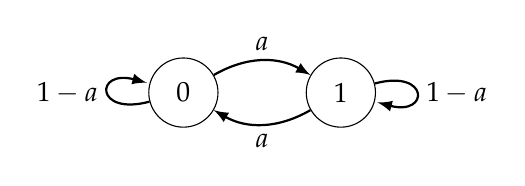
\begin{tikzpicture}[node distance=2cm,->,>=latex,auto,every edge/.append style={thick}]

\node[state] (0) {$0$};
\node[state] (1) [right of=0] {$1$};  

% Arrow from 0 to itself. 
\path (0) edge[loop left]  node{$1-a$} (0)
% From 0 to 1
edge[bend left]  node{$a$}   (1)
% Arrow from 1 to itself.
(1) edge[loop right] node{$1-a$}  (1)
% From 1 to 0.
edge[bend left] node{$a$}     (0);
\end{tikzpicture}
\end{center}


\myspace
\p \blue{Passage of Time}. Flip a coin with $Pr(H) = p$ until we get $H$. \textbf{Question}: How many flips will this take, on average? Define Markov chain:

\begin{center}
	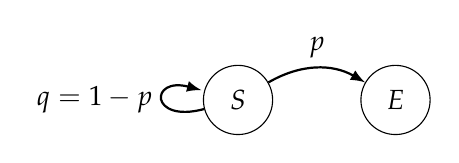
\begin{tikzpicture}[node distance=2cm,->,>=latex,auto,every edge/.append style={thick}]
	\node[state] (0) {$S$};
	\node[state] (1) [right of=0] {$E$};  
	% Arrow from 0 to itself. 
	\path (0) edge[loop left]  node{$q=1-p$} (0)
	% From 0 to 1
	edge[bend left]  node{$p$}   (1);
	\end{tikzpicture}
\end{center}

\begin{compactitem}
	\item $X_0 = S$
	\item $X_n = S$ for $n \ge 1$ if last flip was $T$ and no $H$ yet.
	\item $X_n = E$  for $n \ge 1$ if we already got $H$ (end). 
\end{compactitem}

\textbf{Answer}: $\beta(S)$ be average time until $E$, starting from $S$. Then\footnote{Interpret as ``one unit of time from first step, then with prob $q$ we are back in same state and therefore have $\beta(S)$ time left on average, or with prob $p$ we make it to $E$ and we are done.''} 
\begin{align}
\beta(S) &= 1 + q \times \beta(S) + p \times 0 \\
&= 1/p
\end{align}
This approach is known as a \textit{first-step analysis}. 

\myspace
\p \blue{Dice roll}. You roll a die until the sum of the last two rolls is 8. \textbf{Question}: How many times do you have to roll the die on average?
\begin{compactitem}
	\item \textbf{Draw Markov chain}. Start state points to six possible outcomes of first roll, and each of these points to all possible subsequent states. Note that some of these point to the state E, meaning they have a probability of obtaining the stopping condition on the next roll. 
	
	\item \textbf{First-step equations}. Write out each $\beta(i)$ for all states $i$ in the Markov chain. Note that you can exploit \textit{symmetries},
	\begin{align}
		\beta(1) &= \beta{S} \\
		\beta(2) &= \cdots = \beta(6) = \gamma
	\end{align}
	
	\item \textbf{Solve for $\beta(S)$}. Only unknown is $\gamma$ when we write out $\beta(S)$. Solve by applying the first-step equations from any state $i$ with $\beta(i) = \gamma$ to obtain result as follows.
	\begin{align}
		\beta(S) &= 1 + (5/6) \gamma + \beta(S)/6 \\
		\gamma &= 1 + (4/6)\gamma + (1/6)\beta(S)\\
		\Rightarrow \beta(S) &= 8.4 
	\end{align}
\end{compactitem}


\myspace
\p \blue{Ladder climbing}. Illustrates more general approach. You try to go up a 20 rung ladder, where at each step you move up one rung with prob $p = 0.9$ or you fall all the way back to the bottom. Key idea is to write out the first-step equations in the following general form:
\graybox{
	\beta(n) &= 1 + p \beta(n + 1) + q\beta(0) \qquad 0 \le n  \le 19 \\
	\beta(19) &= 1 + p 0 + q \beta(0) \\
	\Rightarrow \beta(0) &= \frac{p^{-20} - 1}{1 - p}
	}



\myspace
\p \blue{Probability of \$100 before \$0.} Flip biased coin with $P(H) = p < 0.5$, starting with \$10. At each step, if flip yields $H$ you get 1 dollar, else you lose 1 dollar. \textbf{Question:} What is the probability that you reach \$100 \textit{before \$0}?
\begin{compactitem}
	\item \textbf{Approach}: Disregard fact that you 'start' with \$10, it is meant to throw you off. What matters is (1) the possible states you can be in ($0 \le n_i \le 100$) and the transition probabilities.\footnote{Note that the biggest difference b/w this and the other examples is we are looking for a \textit{probability} of reaching some terminal state as opposed to the number of steps before reaching it. Also, there are two terminal states here.} 
	
	\item \textbf{Solution:}\footnote{See Lecture Note 24 for details on solving the equations} Let prob of reaching 100 before 0, starting from some state $n$, be $\alpha(n)$, where $n = 0, 1, \ldots, 100$. Note that the terminal probabilities are $\alpha(0) = 0$ and $\alpha(100) = 1$.
	\graybox{
		\alpha(n) &= p~\alpha(n + 1) + q\alpha(n - 1) \qquad 0 \le n \le 100 \\
		\Rightarrow \alpha(n) &= \frac{1 - \rho^n}{1 - \rho^{100}} \qquad \rho = qp^{-1}
		}
\end{compactitem}

\myspace
\p \blue{Accumulating Rewards}. Let $X_n$ be a Markov chain on $\mathscr{X}$ with $P$. Let $A \subset \mathscr{X}$ and $g:\mathscr{X} \rightarrow \mathcal{R}$ be some [reward] function. 
\graybox{
	\gamma(i) &= \E{ \sum_{n = 0}^{T_A} g(X_n) \mid X_0 = i} \qquad i \in \mathscr{X} \\
	\gamma(i) &= \begin{cases}
		g(i) & \text{if } i \in A \\
		g(i) + \sum_j P(i , j) \gamma(j) & \text{otherwise} 
	\end{cases}
}
Example: Flip fair coin until get 2 consecutive $H$. What is expected number of $T$ we will see? Here is our Markov chain:
\begin{center}
	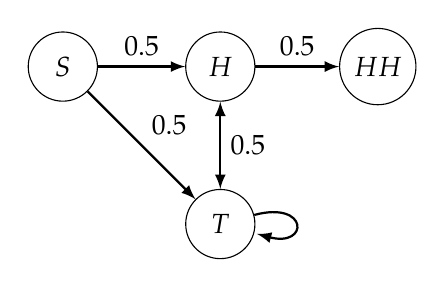
\begin{tikzpicture}[node distance=2cm,->,>=latex,auto,every edge/.append style={thick}]
	\node[state] (S) {$S$};
	\node[state] (H) [right of=S] {$H$};  
	\node[state] (HH)[right of=H] {$HH$};
	\node[state] (T) [below of=H] {$T$};
	\path(S) 
		edge[->] node{$0.5$} (H)
		edge[->]  node{$0.5$} (T);
	\path(H)
		edge[<->] node{$0.5$} (T)
		edge[->]  node{$0.5$} (HH);
	\path(T)
		edge[loop right] (T);
	\end{tikzpicture}
\end{center}
where we define our reward function to yield 1 when we are on $T$ and 0 otherwise\footnote{Recall that reward func $g(i)$ evaluates the reward for us being [currently] on state $i$.}. Our first step equations give us the desired expectation. 
\begin{align}
\gamma(S) &= 0 + 0.5 \cdot \gamma(H) + 0.5 \cdot \gamma(T) \\
\gamma(H) &= 0 + 0.5 \cdot \gamma(HH) + 0.5 \cdot \gamma(T) \\
\gamma(T) &= 1 + 0.5 \cdot \gamma(H) + 0.5 \cdot \gamma(T) \\
\gamma(HH)&= 0 \\
\Rightarrow \gamma(S) &= 2.5
\end{align}

\myspace
\p\hfil\rule{0.7\textwidth}{1pt}\myfig[0.6\textwidth]{MarkovEqs.png}\hfil


% ======================================================================
% CS70: NON Linear Regression
% ======================================================================
\lecture{Discrete Math and Probability}{Markov Chains II}{November 16}

\p \blue{Distribution of $X_n$}. \textbf{Question}: What is the probability that we are in a given state $X_n$ at some time step $m$. To answer, first let $\pi_m(i) = \Pr(X_m = i)$ denote the probability of being in state $i$ at time $m$. Then
\graybox{
	\pi_{m + 1}(j) &= \sum_i \pi_m(i) P(i, j), \qquad \forall j \in \mathscr{X} \\
	\bm{\pi}_{m + 1} &= \bm{\pi}_m \matr{P}
	}
where $P(i, j)$ is the probability of being in $X_{m + 1} = j$ given past $X_m = i$. Note that $\bm{\pi}$ is a row vector here.
\begin{comment}
(maybe not) see [16:00]
	As $m$ increases, $\pi_m$ converges to a vector that does not depend on $\pi_0$. 
\end{comment}

\myspace
\p \blue{Balance Equations}. 
\begin{compactitem}
	\item \textbf{Question}: Is there $\pi_0$ s.t. $\pi_m = \pi_0$, $\forall m$? \green{$\Leftarrow$ Invariant distribution}
	\item \Theorem[A distribution $\pi_0$ is invariant iff $\pi_0 P = \pi_0$]  \green{$\Leftarrow$ Balance equations}
\end{compactitem}
If $\pi_0$ invariant, \emph{distribution} of $X_n$ is always same as $X_0$. Below, we show that this means that the probability of being in some state $j \ne i$ and then entering $i$ is the same as the probability of being in the state $i$ and going to any other state $j \ne i$. 
\begin{align}
	\pi(i) &= \sum_{j} \pi(j) P(j, i) \\
	\sum_{j \ne i} \pi(j) P(j, i) &= \pi(i)(1 - P(i, i)) = \pi(i)\sum_{j \ne i} P(i, j)
\end{align}

\myspace
\p \blue{Irreducibility}. A Markov chain is \textit{irreducible} if it can go from every state $i$ to every state $j$ (possibly in multiple steps). 
\begin{compactitem}[$\rightarrow$]
	\item \textbf{Existence/Uniqueness}. \Theorem[A finite irreducible Markov chain has one and only one invariant distribution]\footnote{That is, there is a unique positive vector $\pi = [\pi(1), \ldots, \pi(K)]$ such that $\pi P = \pi$ and $\sum_k \pi(k) = 1$. See Note 24 or EE126 for proof (apparently impossible to understand)}
	
	\item \textbf{Fraction of Time}. \Theorem[Let $X_n$ be an irreducible Markov chain with invariant distribution $\pi$. Then for all $i$ ]
	\graybox{
		\frac{1}{n}\sum_{m = 0}^{n - 1} 1 \{ X_m = i\} \rightarrow \pi(i), \qquad \text{as } n \rightarrow \infty
		}
\end{compactitem}
Note that having a MC be irreducible does \textit{not} imply that $\pi_n$ approaches the unique invariant distribution $\pi$. 

\myspace
\p \blue{Periodicity}. Assume that the MC is irreducible. Then\footnote{How to get this for a given MC visually for a given state $i$: \begin{compactitem}
		\item \textbf{Build the list}. Find the smallest number of steps needed to reach $i$ again, starting from $i$. Then find the next smallest, and so on and so forth until you have a set of numbers $n > 0$. 
		\item \textbf{Take the gcd} of this set of numbers. 
		\item Try again for some other state $j$. If the MC is irreducible, you're guaranteed to get the same answer for the gcd.
	\end{compactitem}}
\graybox{
	d(i) := \gcd\{ n > 0 ~ | ~ P(X_n = i \mid X_0 = i) > 0 \}
	}
has the same values for all states $i$. If $d(i) = 1$, the MC is said to be \textbf{aperiodic}. Otherwise, it is periodic with period $d(i)$. 
	
\myspace
\p \blue{Convergence of $\pi_n$}. Let $X_n$ be an irreducible and \emph{aperiodic} MC with invariant distribution $\pi$. Then, for all $i \in \mathscr{X}$
\graybox{
	\pi_n(i) \rightarrow \pi(i), \qquad \text{as } n \rightarrow \infty
	}
Note: at \purple{[47:00]}, has slide that may help with programming $\pi$ in Python. 

\myfig[0.3\textwidth]{MarkovEqs2.PNG}



% ======================================================================
% CS70: NON Linear Regression
% ======================================================================
\lecture{Discrete Math and Probability}{Continuous Probability I}{November 18}

\p \blue{Overview}. 
\begin{compactitem}
	\item Examples.
	\item Events.
	\item Continuous Random Variables.
\end{compactitem}

\myspace 
\p \blue{Uniformly at Random in $[0, 1]$}. We describe this by saying
\begin{align}
\Prob{X \in [a, b]} = b - a, \qquad \forall 0 \le a \le b \le 1
\end{align}
where $[a,b]$ denotes the \textbf{event} that the point $X$ is in interval $[a,b]$. More generally, if $A_n$ are pairwise disjoint intervals in $[0, 1]$, then 
\begin{align}
\Prob{\cup_n A_n} := \sum_n \Prob{A_n}
\end{align}
The difference between this and what we've previously done is that we don't start with [individual] \textit{outcomes} (e.g. Pr($\omega$)) but rather we start with \textit{events} (interval subsets of the space). Define $F(x) = \Prob{X \le x}$. Then $$\Prob{X \in (a, b]} = \Prob{X \le b} - \Prob{X \le a} = F(b) - F(a)$$ thus $F(\cdot)$ specifies the probability of all the events. Alternatively, define $f(x) = \deriv{}{x}F(x) = 1 \{x \in [0, 1]\}$. Then 
\graybox{
 F(b) - F(a) &= \int_a^b f(x)\mathrm{d}x \\
 \Prob{X \in A} &= \int_A f(x)\mathrm{d}x
}


\myspace
\p \blue{General Random Choice in $\mathfrak{R}$}. Let $F(x)$ be nondecreasing function, called the \textbf{cumulative distribution function (cdf)} with $F(-\infty) = 0$ and $F(+\infty) = 1$. 
\graybox{
	\Prob{X \in (a_1, b_1] \cup \cdots \cup (a_n, b_n]} &= F(b_1) - F(a_1) + \cdots + F(b_n) - F(a_n) \\
	\Prob{X \in (x, x+ \varepsilon]} &= F(x + \varepsilon_) - F(x) \approx f(x) \varepsilon
	}
where $f(x)$ is the \textbf{probability density function (pdf)}. More on discrete approximation at \purple{[33:00]}


\myspace
\p \blue{Example: Expo($\lambda$)}. The exponential distribution with parameter $\lambda > 0$ is defined by 
\begin{align}
	f_X(x) &= \lambda e^{-\lambda x} ~ 1\{x \ge 0 \} \\
	F_x(x) &= \begin{cases} 0 &  x < 0 \\ 1 - e^{-\lambda x} & x \ge 0 \end{cases}
\end{align}


% ======================================================================
% CS70: Continuous Probability II
% ======================================================================
\lecture{Discrete Math and Probability}{Continuous Probability II}{November 21}

\p \blue{Overview}
\begin{compactitem}
	\item Properties
	\item Expectation
	\item Variance
	\item Independent Continuous RVs
\end{compactitem}



\myspace
\p \blue{Properties}
\begin{itemize}
	\item Expo is \textbf{memoryless}. Let $X = \text{Expo}(\lambda)$. Then, for $s, t > 0$, $\Prob{X > t + s | X > s} = \Prob{X > t}$.
	\item \textbf{Scaling} Expo. Let $X = \text{Expo}(\lambda)$ and $Y = aX$ for some $a > 0$. Then $$\Prob{Y > t} = e^{-\lambda(t/a)} = \Prob{Z > t} \qquad \text{for } Z = \text{Expo}(\lambda/a) $$ and also note that $\text{Expo}(\lambda) = \tfrac{1}{\lambda}\text{Expo}(1)$. 
	
	\item \textbf{Scaling} Unif. Let $X = U[0, 1]$ and $Y = a + bX$ where $b > 0$. 
	\begin{align}
		\Prob{Y \in (y, y + \delta)} &= \Prob{X \in (\frac{y - a}{b}, ~ \frac{y + \delta - a}{b})} \\
		&= \frac{1}{b} \delta \qquad \text{for} \quad a < y < a + b
	\end{align}
	hence $Y = U[a, a + b]$. 
	
	\item \textbf{Scaling} pdf \purple{[19:24]}. Let $f_X(x)$ be pdf of $X$ and $Y = a + bX$ where $b > 0$. Then we can get the pdf of $Y$ via
	\begin{align}
		\Prob{Y \in (y, y + \delta)} &= \Prob{X \in (\frac{y - a}{b}, ~ \frac{y + \delta - a}{b})} = f_X(\frac{y - a}{b})\frac{\delta}{b}\\
		\Rightarrow f_Y(y) &= \frac{1}{b}f_X(\frac{y -a}{b})
	\end{align}
\end{itemize}

\myspace
\p \blue{Expectation}. The \textbf{expecation} of a RV X with pdf $f_X(x)$ is \textit{defined} as 
\graybox{
	\E{X} &= \int_{-\infty}^{\infty} xf_X(x) dx
	}
\textbf{Justification}: For any function $g$, we can approximate its integral via $$\int g(x)dx \approx \sum_n g(n\delta)\delta$$ So, choose $g(x) = x f_X(x)$. \purple{[23:00]}


\myspace
\p \blue{Independent Continuous RVs}. The continuous RVs $X$ and $Y$ are independent if either of the following are true.
\graybox{
	\Prob{X \in A, ~ Y \in B} &= \Prob{X \in A}\Prob{Y \in B} \qquad \forall A, B \\
	f_{X, Y}(x, y) &= f_X(x)f_Y(y)
		}



% ======================================================================
% CS70: Continuous Probability III
% ======================================================================
\lecture{Discrete Math and Probability}{Continuous Probability III}{November 28}


\myspace
\p \blue{Maximum of Two Exponentials}. Let $X = \mathrm{Expo}(\lambda)$ and $Y = \mathrm{Expo}(\mu)$ be independent. Define $Z = \mathrm{max}\{X, Y\}$. \textbf{Calculate} $\E{Z}$. 
\begin{enumerate}
	\item Recall that expo is described by 
	\begin{align}
	f_X(x) &= \lambda e^{-\lambda x} ~ 1\{x \ge 0 \} \\
	F_x(x) &= \begin{cases} 0 &  x < 0 \\ 1 - e^{-\lambda x} & x \ge 0 \end{cases}
	\end{align}
	
	\item Key Idea: Find the CDF, $\Pr(Z \le z)$, then take the derivative to obtain the pdf $f_Z(z)$. Then compute the result as $\E{Z} = \int_{0}^{\infty} z ~ f_Z(z) \mathrm{d}{z}$. 
\end{enumerate}

\myspace
\p \blue{CLT}. Let $X_1, \ldots, X_n$ be i.i.d. with $\E{X_i} = \mu$. Also $A_n = 1/n \sum_i X_i$. Then,
\graybox{
	S_n &:= \frac{A_n - \mu}{\sigma/\sqrt{n}} = \frac{X_1 + \cdots + X_n - n\mu}{\sigma\sqrt{n}} \\
	\Prob{S_n \le \alpha} \quad&\rightarrow\quad \frac{1}{\sqrt{2\pi}} \int_{-\infty}^{\alpha} e^{-x^2/2} dx \qquad \text{(as $n\rightarrow\infty$)}
	}







% _____________________________________________________________________________________________________
% _____________________________________________________________________________________________________
% _____________________________________________________________________________________________________

\clearpage
\appendix 

\mysection{Appendix}

\clearpage
\section*{\Large{Common Series}}
\p \blue{Sums of Powers of First $n$ Integers}
\begin{align}
	\sum_{k = 1}^{n} k &= \dfrac{n (n + 1) }{2} \\
	\sum_{k = 1}^{n} k^2 &= \dfrac{n (n + 1) (2n + 1)}{6} \\
	\sum_{k = 0}^{n - 1} r^k &= \frac{1 - r^n}{1 - r}
\end{align}


\myspace
\section*{\Large{Unintuitive Things I Might Forget}}

\p \blue{Law of Large Numbers (LLN)}. (and coin tosses)
\begin{itemize}
	\item You're actually \textit{less likely} to get \emph{exactly} 50\% Heads for large $n$ compared with any smaller $n$. To show this, compare $P(\text{n heads in 2n tosses})$ with $P(\text{n+1 heads in 2(n+1) tosses})$. 
\end{itemize}

\myspace
\p \blue{Variance/Covariance}. 
\begin{itemize}
	\item If $Cov(X, Y) \ge 0$, $Cov(Y, Z) \ge 0$, it does \textit{not} automatically guarantee that $Cov(X, Z) \ge 0$. 
\end{itemize}

\myspace
\p \blue{Expectation}. 
\begin{itemize}
	\item \textbf{Think in proportions}. If you have $m$ sick people, and the probability that a sick person gets healthy is $\beta$, then the \textit{expected} number of sick people you'll have at the next step is $(1-\beta) m$, since, on average, the fraction of them we would expect to remain sick is $(1 - \beta)$. 
\end{itemize}

\myspace
\p \blue{Markov Chains}. 
\begin{itemize}
	\item When designating rewards, $\gamma(i)$, for each state $i$, make sure to remember that rewards correspond to what you get right when you \textit{arrive to/reach} the state. They should never be multiplied by probabilities, since you are 100\% going to get the reward when you hit the state.
\end{itemize}

\myspace
\p \blue{Continuous Probabilitiy}. 
\begin{itemize}
	\item The probability of some set of i.i.d. RVs, $A, B, \ldots$, all taking on values within some $\delta$ of each other, is
	\begin{align}
		\Pr(\max(A, B, \ldots) - \min(A, B, \ldots) < \delta) 
	\end{align}
\end{itemize}


\clearpage
\section*{\Large{Problems to Review}}

\p \blue{Spring 2016 Final}. \href{https://d1b10bmlvqabco.cloudfront.net/attach/irwxcmgdofp2uz/hzcyh0n929z1id/iwgoqrni6gl7/cs70_sp16_f_sol.pdf}{Link to solutions.}
\begin{compactitem}
	\item Problem 3.4. Particularly part (c). It seems like the underlying logic here is that $\E{X_n} \rightarrow pN$ as $n \rightarrow \infty$ suggests that 
\end{compactitem}

\myspace
\hrule\hrule
\section*{\Large Cool Extra Concepts}

\begin{compactitem}
	\item \textbf{Free Space}: the vector space of random variables is the vector space of functions $X:\Omega\rightarrow\R$, also called the \textit{free space} of $\R$ over the set $\Omega$.
\end{compactitem}
\myspace
\hrule\hrule




\begin{align}
\Var{Unif\{1, \ldots, n\}} = \frac{n^2 - 1}{12}
\end{align}





























\end{document}

































% fuck
